\documentclass[12pt
,a4paper
,titlepage
,twoside
%,openany % ouvre les sections indifféremment sur la page de gauche ou de droite
]{book}

% Définition des marges de la page
\usepackage[left=3cm,right=3cm,top=2cm,bottom=2cm]{geometry}

% Paramétrages de la langue et de l'encodage
\usepackage[utf8x]{inputenc}
\usepackage[square,sort,comma,numbers]{natbib}
\usepackage[french]{babel}
\usepackage[T1]{fontenc}

%\usepackage{fontspec}
%\setmainfont{Linotype-AvenirNextLTPro.ttf}[
%BoldFont = Linotype-AvenirNextLTProBold.ttf,
%ItalicFont = Linotype-AvenirNextLTProItalic.ttf,
%BoldItalicFont = fLinotype-AvenirNextLTProBoldItalic.ttf
%]

% formules mathématiques
\usepackage{amsmath}
\usepackage{amsfonts}
\usepackage{amssymb}

% gestion des graphiques
\usepackage{graphicx}
\usepackage{transparent}

% Gestion des couleurs
\usepackage[usenames,dvipsnames]{xcolor}
\definecolor{inrae}{RGB}{0,163,166} % inrae
\definecolor{inraeclair}{RGB}{102,193,191}   % inrae clair
\definecolor{inraemedium}{RGB}{0,140,142}   % inrae medium
\definecolor{inraefonce}{RGB}{39,86, 98} % inrae foncé
\definecolor{vert}{RGB}{157,197,68} % vert
\definecolor{bleuclair}{RGB}{158,214,227} % bleu clair
\definecolor{bleufonce}{RGB}{66,48,137} % bleu foncé
\definecolor{gris}{RGB}{121,120,112}   % gris
\definecolor{argent}{RGB}{196,192,179} % argent
\definecolor{rouge}{RGB}{142,2,0} % rouge

% Redefinition des liens web
\usepackage{url}
\usepackage{hyperref}
\hypersetup{
urlcolor=inraefonce
,linkcolor=.
,colorlinks=true}


% Polices de caractères
\usepackage{times}
\usepackage{mathptmx} % times, y compris dans les formules mathématiques
\renewcommand{\familydefault}{\sfdefault}

% Insertion de code source dans le texte, à utiliser avec \begin{lstlisting} et \lstset{java|html|php...}
\usepackage{listings}
\lstset{
basicstyle=\footnotesize,        % the size of the fonts that are used for the code
  breakatwhitespace=false,         % sets if automatic breaks should only happen at whitespace
  breaklines=true,
  keepspaces=true,
}

% Définition des entêtes
\usepackage{fancyhdr}
\pagestyle{fancy}

% Redéfinition des titres de section
\usepackage{titlesec}

% Insertion de graphiques à des emplacements définis
\usepackage[abs]{overpic}

% règles typographiques de l'Imprimerie nationale
\usepackage[all]{nowidow}
\usepackage[
% frenchchapters renomme le premier chapitre, mais :
%	- cela pose problème dans la table des matières
%	- cela ne peut être utilisé qu'avec la renumérotation des chapitres activée
%frenchchapters,
parindent,
lastparline,
hyphenation
]{impnattypo}

% Renumérotation des chapitres
%\renewcommand{\thesection}{\Alph{section})}
%\renewcommand{\thesubsection}{\arabic{subsection} -}
%\renewcommand{\thesubsubsection}{\alph{subsubsection} -}
%\usepackage{engrec}
%\renewcommand{\theparagraph}{\engrec{paragraph})}
%\setcounter{secnumdepth}{4}

% Génération du code Ipsum lorem
\usepackage{blindtext}


% Definition des chapitres
%\usepackage{sectsty}
\titleformat{\chapter}[display]
{\normalfont\Huge\filcenter\sffamily\color{inrae}}
{\Large{\chaptertitlename~\thechapter}}
 {1em}{}

%{\titlerule
%% \vspace{1pc}%


\titleformat{\section}
{\color{inrae}\normalfont\Large\bfseries\sffamily}
{\color{inrae}\thesection}{1em}{}

\titleformat{\subsection}
{\color{inraefonce}\bfseries\sffamily}
{\color{inraefonce}\thesubsection}{1em}{}

\titleformat{\subsubsection}
{\color{gris}\bfseries\sffamily}
{\color{gris}\thesubsubsection}{1em}{}

% Bibliographie
% natbib est indispensable si la biblio contient des accents
% Options pour natbib (extrait de http://merkel.zoneo.net/Latex/natbib.php)
%    round: (par défaut) pour des parenthèses arondies (());
%    square: pour des crochets ([]);
%    curly: pour des accolades ({});
%    angle: pour des équerres (<>) ;
%    colon: (par défaut) pour séparer les citations multiples par deux points (:);
%    comma: pour utiliser une virgule comme séparateur;
%    authoryear: (par défaut) pour des citations auteurs-année;
%    numbers: pour des citations numériques;
%    super: pour des citations numériques en exposant, comme dans Nature;
%    sort: ordonne les citations multiples dans l'ordre dans lequel elles apparaissent dans la bibliographie;
%    sort&compress: comme sort mais en plus les citations numériques multiples sont comprimées, si possible (3-6, 15, par exemple);
%    longnamesfirst: transforme la première citation à une référence en une version étoilée (avec la liste complète des auteurs) et le citations suivantes normales (liste abbrégée);
%    sectionbib: pour redéfinir \thebibliography pour avoir une \section* à la place d'un \chapter*; valide seulement pour les classes de document possédant la commande \chapter; à utiliser avec le paquetage  chapterbib;
%    nonamebreak: garde tous les noms d'auteurs d'une citation sur une même ligne; celà cause des problèmes de débordement, mais permet de résoudre certains problèmes liés à hyperref.

% En cas de souci, supprimez les fichiers .aux et .bbi après modification des paramètres
% styles natbib natifs : abbrvnat, plainnat, unsrtnat
\bibliographystyle{unsrtnat}
\usepackage{hypernat}
% Ajout de la référence à la bibliographie dans la table des matières
\usepackage[nottoc, notlof, notlot]{tocbibind}

%Données de titre et d'auteur pour la page de garde
\newcommand{\titre}{Logiciel Collec-Science}
\newcommand{\sousTitre}{Installation, configuration et administration}
\newcommand{\auteur}{Éric Quinton}
\newcommand{\dateVersion}{1\ier{} août 2022}
\newcommand{\version}{Version 2.8.0}
\usepackage[final]{pdfpages} 

\usepackage{lscape}
\usepackage{longtable}
\usepackage{float}
\usepackage{array}
\begin{document}
%Supprime les veuves et orphelines
\widowpenalty=10000
\clubpenalty=10000
\raggedbottom 

% Integrer la page de garde

\thispagestyle{empty}
\newgeometry{left=2cm,bottom=0.1cm}
\vspace*{4cm}
\textcolor{inrae}{\sffamily\Huge\bfseries\titre}\par
\textcolor{inrae}{\sffamily\Large\bfseries\sousTitre}\par
\textcolor{inrae}{\sffamily\dateVersion{} -- \version}\par

% Sigle INRAE
\vspace*{3cm}

\includegraphics{inrae}\par\bigskip
\textcolor{inrae}{\sffamily\Large Institut national de recherche pour}\par
\textcolor{inrae}{\sffamily\Large\bfseries l'agriculture, l'alimentation et l'environnement}\par\bigskip

% Logo INRAE

\vspace*{2cm}
\hspace{-5cm}
{\transparent{0.4}
\includegraphics[width=10cm]{sigle-inrae-plein}}

\vspace*{2cm}
   \textcolor{inrae}{\sffamily
   Site web de Collec-Science :
   {\large \href{https://www.collec-science.org}{https://www.collec-science.org} }
   }\par
\vspace*{1cm}
\textcolor{inrae}{\sffamily\auteur}\par

\textcolor{inrae}{\sffamily
Document distribué sous licence CC-BY}\par
  
\includegraphics[width=1cm]{cc-by} \href{https://creativecommons.org/licenses/by/4.0/fr/legalcode}{https://creativecommons.org/licenses/by/4.0/fr/legalcode}
\restoregeometry
% Définition des entêtes
\fancyhead{}
\fancyhead[CO]{\leftmark\sffamily}
\fancyhead[CE]{ \sffamily\titre{}}
\fancyfoot[CO]{\sffamily\thepage}
\fancyfoot[CE]{\sffamily\thepage}
% Redéfinition de \cleardoublepage pour créer une page totalement vide
\makeatletter
\def\cleardoublepage{\clearpage\if@twoside \ifodd\c@page\else
  \hbox{}
  \vspace*{\fill}

  \vspace{\fill}
  \thispagestyle{empty}
  \newpage
  \if@twocolumn\hbox{}\newpage\fi\fi\fi}
\makeatother

% \cleardoublepage permet de générer une page vide 
% si le chapitre ne commence pas sur la page de droite

% Ajout d'un préambule
\frontmatter
\cleardoublepage

% Table des matières
\tableofcontents


% Début réel du texte
\mainmatter
%\cleardoublepage

\chapter{Le logiciel Collec-Science}
\section{Historique}

L'unité de recherche \textit{Écosystèmes aquatiques et changements globaux} d'IRSTEA, à Cestas (33), récolte et manipule des échantillons prélevés sur le terrain (ou plutôt, principalement dans l'eau -- estuaires, lacs, rivières...), et les stocke, parfois pour des durées très longues : certaines campagnes de collecte ont eu lieu il y a plus de 40 ans.

De plus en plus, des échantillons anciens sont réanalysés (analyses génétiques, étude des ossements des oreilles ou otolithes...), au gré des questions scientifiques à traiter. 
Le besoin de recourir à un logiciel pour gérer ces matériels est devenu une priorité.

Dans un premier temps, quelques logiciels open-source susceptibles d'être utilisés ont été étudiés. Toutefois, leurs limites sont vite apparues : problème de pérennité, ancienneté du code, modèle de distribution parfois insatisfaisant (une licence open-source est obligatoire pour assurer la pérennité à longue échéance), résistance aux attaques informatiques, fonctionnalités insuffisantes ou inadaptées au besoin.

Dans un second temps, une étude des besoins réels a été menée. De nouvelles fonctionnalités ont été rajoutées, comme la gestion du stock de matériel utilisé sur le terrain, stocké dans un hangar.

L'unité de recherche s'intégrant au niveau régional avec d'autres organismes, des collaborations avec l'Observatoire Aquitain des Sciences de l'Univers (OASU) ou l'université de La Rochelle ont été envisagées.
Des échanges productifs ont ainsi pu être mis en place, entre autres sur la gestion de l'étiquetage et le scannage des codes-barres.

Le logiciel a largement évolué suite à ces échanges, de nombreuses fonctionnalités ont été rajoutées ou modifiées pour tenir compte des besoin des partenaires potentiels. 

Les délais de développement de la première version opérationnelle se sont étalés sur 9 mois, entre la définition des besoins et le développement proprement dit. 
La première version est parue à l'automne 2016, la version 2.0 est sortie en mai 2018.

Le code comprend environ 15800 lignes (commentaires compris), dont 7600 concernent l'affichage des pages web. Il a été écrit en PHP, les pages web sont générées en HTML et Javascript avec le composant Smarty.

\section{Fonctionnalités générales}

\begin{figure}[H]
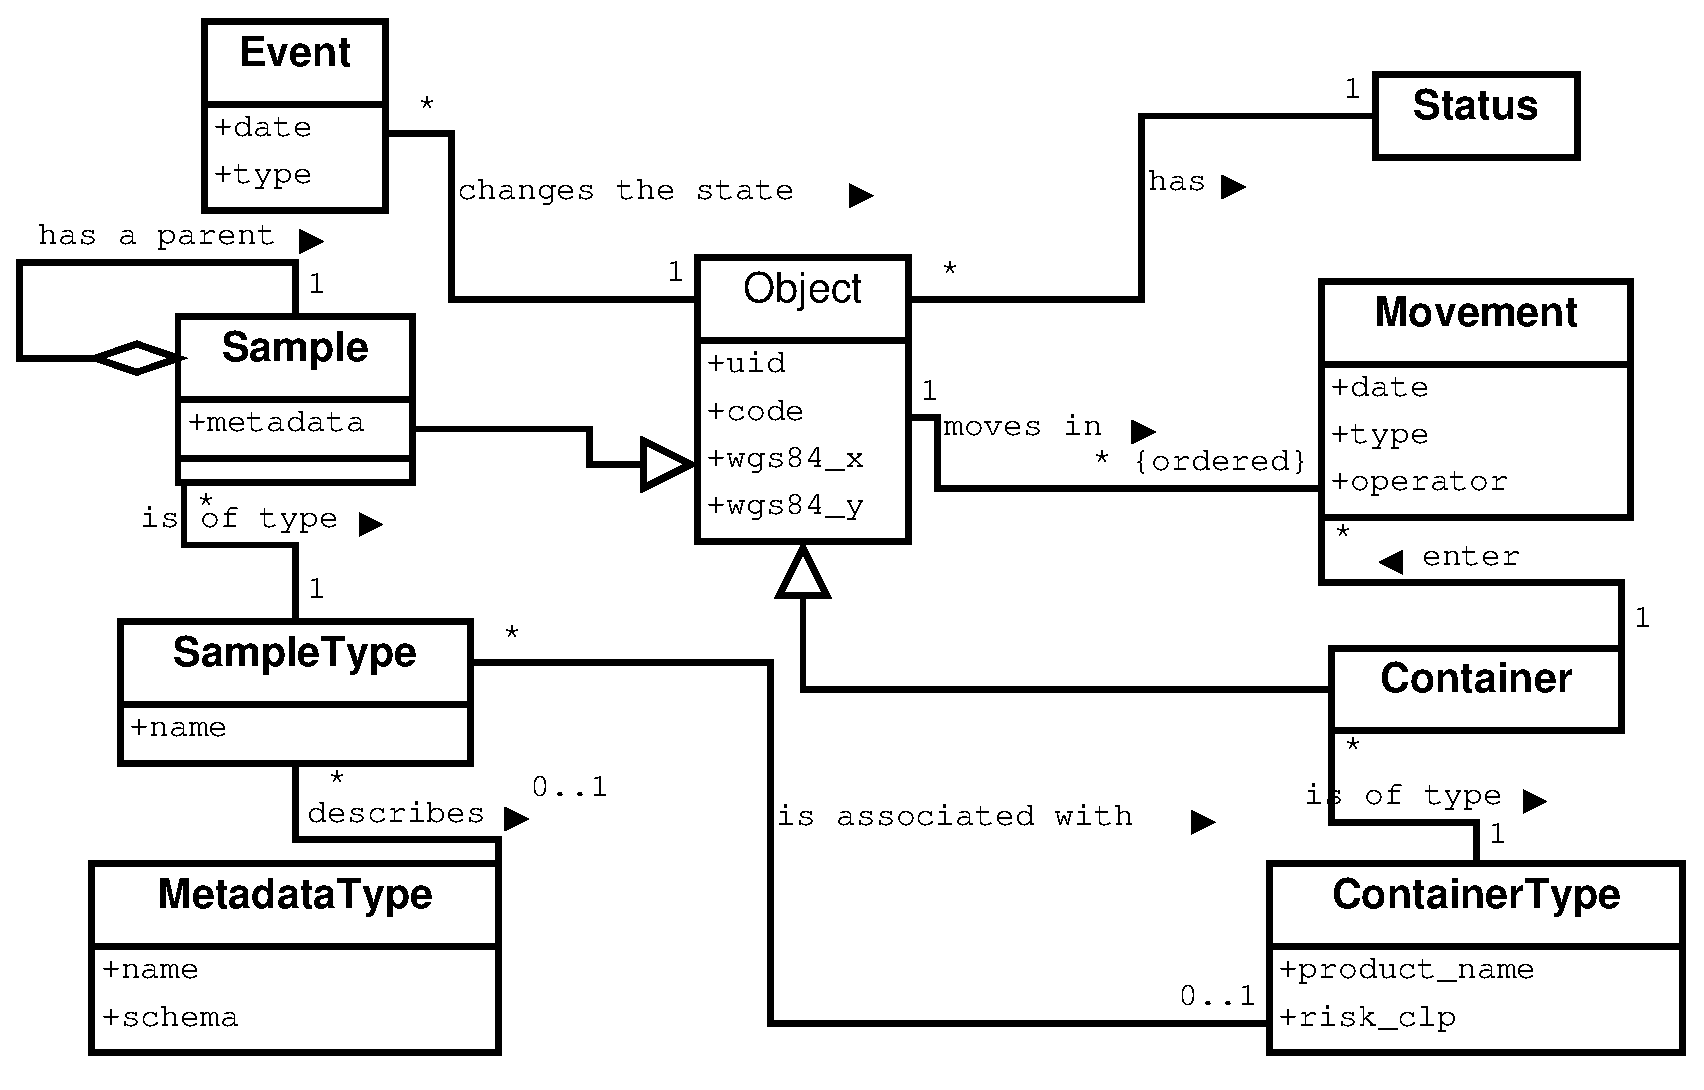
\includegraphics[width=\linewidth]{images/classes2}
\caption{Représentation objet de la base de données}
\end{figure}


Deux types d'objets sont manipulés dans l'application :
\begin{itemize}
\item des conteneurs (container), qui peuvent contenir des objets de tout type : d'autres conteneurs ou des échantillons. Ils peuvent être de différentes nature : site, bâtiment, salle, armoire, caisse, éprouvette... Les types de conteneurs décrivent également le produit de conservation utilisé et le risque associé (brûlure, cancérogène, etc.) ;
\item des échantillons (sample), qui peuvent être associés à un type de conteneur : il y a de nombreux cas où l'échantillon lui-même se confond avec son contenant, par exemple quand le résultat d'une pêche n'est pas trié et est stocké dans un bocal.
\end{itemize}

Un échantillon ou un conteneur sont issus d'un objet unique, qui est doté :
\begin{itemize}
\item d'un numéro unique, l'\textbf{UID}, qui sert de référence dans le logiciel ;
\item d'un identifiant métier, qui servira à le retrouver facilement (le logiciel permet également de définir d'autres identifiants).
\end{itemize}

Un objet peut subir un certain nombre d'événements, voire être réservé (fonctionnalité très simplifiée, seul le recouvrement de deux périodes de réservation est signalé).

Tout objet peut être étiqueté. Les étiquettes peuvent comprendre un code-barre 2D de type QRCode, qui pourra être lu soit à partir d'un terminal dédié (douchette), soit avec une tablette ou un smartphone, l'application disposant d'un module capable d'activer la caméra depuis le navigateur et de scanner le code-barre.

Un échantillon est obligatoirement rattaché à une collection. Seuls les les personnes rattachées à celle-ci peuvent modifier les informations le concernant. 

Pour mieux décrire les échantillons, il est possible de leur rattacher quelques informations \og métier \fg{}, appelées ici \textit{métadonnées}. Les types de métadonnées, totalement paramétrables, sont rattachés aux types d'échantillons.

Un échantillon peut être subdivisé en d'autres échantillons. Par exemple, des otolithes (os de l'oreille) peuvent être extraits d'un poisson. Le logiciel permet de créer un nouvel échantillon à partir d'un autre, qui peut être d'un autre type le cas échéant, et qui restera associé au parent. 

Enfin, dans certains cas de figures, un échantillon peut être composé de plusieurs éléments indifférenciés, par exemple plusieurs écailles de poisson prélevées et conservées ensemble. Le logiciel permet d'indiquer les prélèvements et les restitutions réalisées, et affiche le solde (théorique !) restant.

\section{Technologie employée}
\subsection{Base de données}

L'application a été conçue pour fonctionner avec Postgresql, en version 9.5. Les versions antérieures peuvent être utilisées, mais seule cette version dispose d'un type de données JSON qui permet de stocker les informations métiers.

\subsection{Langage de développement et framework utilisé}
Le logiciel a été écrit en PHP, en s'appuyant sur le framework \textit{Prototypephp} \cite{prototypephp}, développé parallèlement par l'auteur du logiciel.

Il utilise la classe \textit{Smarty} \cite{smarty} pour gérer l'affichage des pages HTML. Celles-ci sont générées en utilisant \textit{Jquery} \cite{jquery}  et divers composants associés. Le rendu général est réalisé avec \textit{Bootstrap} \cite{bootstrap}.

Les étiquettes sont générées en utilisant FOP \cite{fop}, une classe Java qui crée des fichiers PDF à partir d'un fichier XML contenant les données et un fichier de transformation au format XSL.

\subsection{Liste des composants externes utilisés}

\begin{longtable}{|>{\raggedright\arraybackslash}p{3cm}|c|c|>{\raggedright\arraybackslash}p{3cm}|>{\raggedright\arraybackslash}p{3cm}|}
\hline 
\textbf{Nom} & \textbf{Version} & \textbf{Licence} & \textbf{Usage} & \textbf{Site} \\ 
\hline 
\endhead
PrototypePHP & branche bootstrap & LGPL & Framework & \href{https://github.com/equinton/prototypephp}{github.com/ equinton/ prototypephp} \\ 
Smarty & 3.1.31 & LGPL & Générateur de pages HTML & \href{http://www.smarty.net}{www.smarty.net} \\ 
Smarty-gettext & 1.2.0 & LGPL & Support multi-langues pour Smarty & \\
PHPCAS & 1.3.5 & Apache 2.0 & Identification auprès d'un serveur CAS & \href{https://wiki.jasig.org/display/CASC/phpCAS}{wiki.jasig.org/ display/ CASC/ phpCAS} \\ 
PHPQRCODE &  1.1.4 & LGPL & Génération des qrcodes & \\
Zxcvbn-PHP & 0.3 & MIT & Vérification de la complexité des mots de passe & \\

\hline 
\caption{Table des composants PHP externes utilisés dans l'application}
\end{longtable} 

\begin{longtable}{|>{\raggedright\arraybackslash}p{3cm}|c|c|>{\raggedright\arraybackslash}p{3cm}|>{\raggedright\arraybackslash}p{3cm}|}
\hline 
\textbf{Nom} & \textbf{Version} & \textbf{Licence} & \textbf{Usage} & \textbf{Site} \\ 
\hline 
\endhead
Bootstrap & 3.0 & MIT & Présentation HTML & \href{http://getbootstrap.com}{get.bootstrap.com} \\ 
ComboBox & 1.0.1 & MIT & gestion des combobox & \\

JavaScript Cookie & 2.1.4 & MIT & Gestion des cookies dans le navigateur & \href{https://github.com/js-cookie/js-cookie}{github.com/ js-cookie/ js-cookie} \\ 

Datatables & 1.10.20 & MIT & Affichage des tableaux HTML & \href{http://www.datatables.net/}{www.datatables. net} \\ 

Datetime-moment &  & MIT & Formatage des dates dans les tableaux & \href{https://datatables.net/plug-ins/sorting/datetime-moment}{datatables.net/ plug-ins/ sorting/ datetime-moment} \\ 

Moment &  & MIT & Composant utilisé par datetime-moment & \href{http://momentjs.com} {momentjs.com}\\ 

JQuery & 3.3.1 & $\approx$ BSD & Commandes Javascript & \href{http://jquery.com/}{jquery.com} \\ 

JQuery-ui & 1.12.1 & $\approx$ BSD & Commandes Javascript pour les rendus graphiques & \href{http://jqueryui.com/}{jqueryui.com} \\ 

js.cookies & 0.0.4 & & Gestion des cookies & \\

leaflet & 1.3.4 & & Affichage des cartes OpenStreetMap & \\
leaflet-draw & 1.0.4 & & Dessin de polygones sur les cartes & \\
leaflet-mouse-position & 1.2.0 & & récupération de la position de la souris & \\
leaflet-marker-cluster & 1.4.1 & & & \\
leaflet-tylelayer-pouchdbcached & 1.0.0 & & Mise en cache de la cartographie & \\
pouchdb & 7.1.1 & & moteur de mise en cache & \\

Jquery-timepicker-addon &  & MIT & Time picker & \href{https://github.com/trentrichardson/jQuery-Timepicker-Addon}{github.com/ trentrichardson/ jQuery-Timepicker-Addon} \\ 

Magnific-popup & 1.1.0 & MIT & Affichage des photos & \href{http://dimsemenov.com/plugins/magnific-popup/}{dimsemenov .com/plugins/ magnific-popup/}\\ 

Smartmenus & 1.1.0 & MIT & Génération du menu HTML & \href{http://www.smartmenus .org}{www.smartmenus .org} \\ 
 
Openlayers & 4.2.0 & BSD & Affichage des cartes & \href{http://openlayers.org/}{openlayers.org} \\ 

qcode-decoder & & MIT & lecture de codes barres & \href{http://cirocosta.github.io/qcode-decoder/}{cirocosta.github .io/qcode-decoder}\\

Html5-qrcode &  & MIT & Lecture des QRcodes &  \href{https://github.com/dwa012/html5-qrcode}{github.com/ dwa012/ html5-qrcode} \\ 

AlpacaJS & 1.5.23 & Apache 2 & Génération et saisie des métadonnées & 
\href{http://www.alpacajs.org/}{www.alpacajs.org}\\

handlebars & 4.5.3 & & Gestion des boutons dans AlpacaJS & \\
zxcvbn & 4.4.2 & & Vérification de la complexité des mots de passe & \\
\hline
\caption{Table des composants Javascript externes utilisés dans l'application}
\end{longtable} 

\section{Sécurité}

L'application a été conçue pour résister aux attaques dites opportunistes selon la nomenclature ASVS v3 \cite{asvs} de l'OWASP \cite{owasp}. Des tests d'attaque ont été réalisés en août 2016 avec le logiciel ZAProxy \cite{zaproxy}, et n'ont pas détecté de faiblesse particulière.

La gestion des droits est conçue pour :
\begin{itemize}
\item qu'un utilisateur, membre d'une collection, ne puisse modifier que les échantillons qui y sont rattachés ;
\item que tout utilisateur disposant des droits de gestion peut procéder à une entrée ou une sortie d'un objet, quel qu'il soit ;
\item que les responsables d'une collection soient les seuls à pouvoir modifier les paramètres comme les types d'échantillons ou de conteneurs, les protocoles ou les opérations rattachées.
\end{itemize}
L'analyse de sécurité a mis en exergue un besoin de ne pas perdre d'information : si un échantillon est étiqueté et rangé, et que l'information est perdue, il y a de gros risques de ne plus pouvoir l'utiliser ultérieurement. Cela impose la mise en place d'un mécanisme de réplication de la base de données, à implémenter -- ou faire implémenter par des administrateurs du système -- directement dans Postgresql.

\section{Licence}
Le logiciel est diffusé selon les termes de la licence GNU AFFERO GENERAL PUBLIC LICENSE version 3, en date du 19 novembre 2007 \cite{agpl}.

\section{Copyright}

L'application a été déposée par IRSTEA auprès de l'Agence de protection des programmes \cite{app}, sous le numéro IDDN.FR.001.470013.000.S.C.2016.000.31500


\chapter{Installer le logiciel}

\section{Consultez la documentation du framework !}

Le logiciel a été conçu à partir du framework \textit{Prototypephp}. La documentation associée \cite{pphp-doc} récapitule l'ensemble des informations nécessaires pour réaliser l'installation générale (configuration du serveur, définition des droits d'accès, etc.).

De nombreuses passages ont été repris ici, mais il n'est pas inutile de se référer au document d'origine. 

\section{Installation automatique}
Le logiciel est livré avec un script qui installe automatiquement les paquets nécessaires, télécharge le code de l'application depuis Github, crée la base de données et prépare la configuration du serveur web Apache.

L'installateur est conçu pour fonctionner avec une distribution Debian ou Ubuntu (version LTS).

\subsection{Mode opératoire}
\begin{itemize}
	\item installez une distribution Linux (préférentiellement, la dernière Debian stable) ;
	\item connectez-vous en mode \textit{root} ;
	\item téléchargez le script d'installation : \href{https://github.com/Irstea/collec/raw/master/install/deploy_new_instance.sh}{deploy\_new\_instance.sh} avec la commande :
	\begin{lstlisting}
	wget https://github.com/collec-science/collec-science/raw/master/install/deploy_new_instance.sh
	chmod +x deploy_new_instance.sh
	\end{lstlisting}
	\item exécutez le script, qui va réaliser l'ensemble des opérations automatisables ;
	\item éditez ensuite le fichier /etc/apache2/sites-available/collec-science.conf, pour positionner correctement le dns de votre application et indiquer les informations liées au certificat https (clé privée, certificat, autorité de certification) ;
	\item activez le site, puis rechargez Apache :
	\begin{lstlisting}
	a2ensite collec-science
	systemctl reload apache2
	\end{lstlisting}
\end{itemize}

\section{Installation manuelle}
\subsection{Configurer le serveur}

L'application est conçue pour fonctionner à partir d'une adresse unique de type : {\NoAutoSpacing\textit{https://monsite.com}}. Le chiffrement est obligatoire (protocole https). Il n'est pas possible d'installer l'application dans un sous-dossier, par exemple : \linebreak{\NoAutoSpacing \textit{https://monsite.com/collec-science}} ne fonctionnera pas.


\subsection{Configurer Apache}
Les modules suivants doivent être activés :
\begin{lstlisting}
a2enmod ssl
a2enmod headers
a2enmod rewrite
\end{lstlisting}

\subsection{Modules PHP nécessaires}
PHP doit être en version 7.4 au minimum. Il est préférable d'installer PHP depuis le site de PHP plutôt que d'utiliser les paquets fournis par la distribution.

Depuis la version 2.8.0, l'application fonctionne également avec php 8.1.

Modules complémentaires nécessaires (les versions sont en général à indiquer après \textit{php}) :
\begin{itemize}
\item \textit{php-ldap}
\item \textit{php-mbstring}
\item \textit{php-pgsql}
\item \textit{php-xml} 
\item \textit{php-xdebug} pour les phases de mise au point
\item \textit{php-curl} pour l'identification via un serveur CAS
\item \textit{php-zip}
\item \textit{php-imagick}
\item \textit{php-gd}

\end{itemize}
La génération des étiquettes nécessite les paquetages suivants :
\begin{itemize}
\item \textit{fop} (qui inclut des bibliothèques java)
\end{itemize}


\subsection{Installer et configurer php}
Voici le script d'installation automatique qui permet d'installer PHP :

\begin{lstlisting}
#!/bin/bash
PHPVER=8.1

# installing php repository
apt -y install lsb-release apt-transport-https ca-certificates
DISTRIBCODE=`lsb_release -sc`
DISTRIBNAME=`lsb_release -si`
wget -O /etc/apt/trusted.gpg.d/php.gpg https://packages.sury.org/php/apt.gpg
if [ $DISTRIBNAME == 'Ubuntu' ]
then
 # Ubuntu
 apt-get -y install software-properties-common
 add-apt-repository -y ppa:ondrej/php
 add-apt-repository -y ppa:ondrej/apache2
else
# Debian
 wget -q https://packages.sury.org/php/apt.gpg -O- | apt-key add -
 echo "deb https://packages.sury.org/php/ $DISTRIBCODE main" | tee /etc/apt/sources.list.d/php.list
 apt-get update
fi
apt-get -y install libapache2-mod-php$PHPVER php$PHPVER php$PHPVER-ldap php$PHPVER-pgsql php$PHPVER-mbstring php$PHPVER-xml php$PHPVER-zip php$PHPVER-imagick php$PHPVER-gd php$PHPVER-curl
/usr/sbin/a2dismod php$PHPOLDVERSION
/usr/sbin/a2enmod php$PHPVER
# update php.ini
PHPINIFILE="/etc/php/$PHPVER/apache2/php.ini"
upload_max_filesize="=100M"
post_max_size="=50M"
max_execution_time="=120"
max_input_time="=240"
memory_limit="=1024M"
max_input_vars="10000"
for key in upload_max_filesize post_max_size max_execution_time max_input_time memory_limit
do
 sed -i "s/^\($key\).*/\1 $(eval echo \${$key})/" $PHPINIFILE
done
sed -i "s/; max_input_vars = .*/max_input_vars=$max_input_vars/" $PHPINIFILE

# adjust php.ini values
upload_max_filesize="=100M"
post_max_size="=50M"
max_execution_time="=120"
max_input_time="=240"
memory_limit="=1024M"
max_input_vars="10000"
for key in upload_max_filesize post_max_size max_execution_time max_input_time memory_limit
do
 sed -i "s/^\($key\).*/\1 $(eval echo \${$key})/" $PHPINIFILE
done
sed -i "s/; max_input_vars = .*/max_input_vars=$max_input_vars/" $PHPINIFILE
systemctl restart apache2

 adjust imagick policy
sed -e "s/  <policy domain=\"coder\" rights=\"none\" pattern=\"PDF\" \/>/  <policy domain=\"coder\" rights=\"read|write\" pattern=\"PDF\" \/>/" /etc/ImageMagick-6/policy.xml > /tmp/policy.xml
cp /tmp/policy.xml /etc/ImageMagick-6/
\end{lstlisting}


\subsection{Configurer l'hôte virtuel et SSL}
L'application ne fonctionne qu'en mode SSL, les cookies de session n'étant pas transmis sur des liens non chiffrés. Voici un exemple de configuration à insérer dans le fichier \textit{/etc/apache2/sites-available/default-ssl}
\begin{lstlisting}
    <Directory /var/www/html>
        Options FollowSymLinks MultiViews
        AllowOverride all
        Order allow,deny
        allow from all
    </Directory>
SSLProtocol             all -SSLv3
SSLCipherSuite          ECDHE-ECDSA-CHACHA20-POLY1305:ECDHE-RSA-CHACHA20-POLY1305:ECDHE-ECDSA-AES128-GCM-SHA256:ECDHE-RSA-AES128-GCM-SHA256:ECDHE-ECDSA-AES256-GCM-SHA384:ECDHE-RSA-AES256-GCM-SHA384:DHE-RSA-AES128-GCM-SHA256:DHE-RSA-AES256-GCM-SHA384:ECDHE-ECDSA-AES128-SHA256:ECDHE-RSA-AES128-SHA256:ECDHE-ECDSA-AES128-SHA:ECDHE-RSA-AES256-SHA384:ECDHE-RSA-AES128-SHA:ECDHE-ECDSA-AES256-SHA384:ECDHE-ECDSA-AES256-SHA:ECDHE-RSA-AES256-SHA:DHE-RSA-AES128-SHA256:DHE-RSA-AES128-SHA:DHE-RSA-AES256-SHA256:DHE-RSA-AES256-SHA:ECDHE-ECDSA-DES-CBC3-SHA:ECDHE-RSA-DES-CBC3-SHA:EDH-RSA-DES-CBC3-SHA:AES128-GCM-SHA256:AES256-GCM-SHA384:AES128-SHA256:AES256-SHA256:AES128-SHA:AES256-SHA:DES-CBC3-SHA:!DSS
SSLHonorCipherOrder     on
SSLCompression          off
SSLSessionTickets       off

\end{lstlisting}

(attention : pas d'espace entre \textit{Order allow} et la virgule).

La chaîne \textit{SSLCipherSuite} est celle qui fonctionne avec Apache 2.4.24 et openssl 1.1.0f, et est issue du configurateur mis à disposition par la fondation Mozilla \cite{mozillagenerator}. 
Vous pouvez également consulté le document édité par l'ANSSI \cite{tls}. 

Activez ensuite le mode SSL dans Apache :
\begin{lstlisting}
a2ensite default-ssl
service apache2 restart
\end{lstlisting}

\subsection{Configurer Apache pour l'identification à partir d'une fédération}
\label{mellon}
À partir de la version 2.4.0, Collec-Science permet d'identifier les utilisateurs à partir d'une fédération d'identités, comme la fédération française RENATER ou EDUGAIN (la fédération internationale des instituts universitaires et de recherche).

Cette identification n'est possible que pour les applications accessibles depuis Internet, et s'appuie sur l'utilisation d'un module Apache dédié : \textit{Mellon}. Elle nécessite également de récupérer les informations techniques liées à la fédération, et d'enregistrer l'application chez le fournisseur de l'identification.

\subsubsection{Installation du module Mellon}
\begin{lstlisting}
apt-get install libapache2-mod-auth-mellon
\end{lstlisting}

Si le paquet libapache2-mod-auth-mellon n'est pas disponible (cas rencontré avec une distribution Debian \textit{strech}), vous devrez récupérer et installer les paquets suivants (dans l'ordre) :
\begin{itemize}
	\item libxmlsec1
	\item libxmlsec1-openssl
	\item liblasso3
	\item libapache2-mod-auth-mellon
\end{itemize}

Vous devrez également récupérer le fichier xml de votre \textit{provider}, ainsi que son certificat.

\subsubsection{Génération des fichiers de configuration de l'application}
Un certificat (et sa clé privée), un fichier xml doivent être générés pour l'application. Un script est disponible dans les distributions Debian. Il est également fourni dans l'application, dans le dossier install/apache2 (\textit{create\_metadata.sh}).

Pour générer les fichiers (remplacez \textit{collec-science.com} par vos propres valeurs) : 
\begin{lstlisting}
cd /etc/apache2
mkdir mellon
cd mellon
/var/www/html/collec-science/collec/install/apache2/create_metadata.sh https://collec-science.com https://collec-science.com/mellon
\end{lstlisting}

Le certificat (fichier .cert) et le fichier xml doivent être transmis au \textit{provider}, pour qu'il les intègre dans sa plate-forme.

Vous devez également récupérer du \textit{provider} sa clé publique et son certificat d'autorité racine, à mettre dans le dossier \textit{mellon}. Il doit également vous fournir un fichier xml qui contient les adresses de toutes les entités participant à la fédération.

\subsubsection{Configurer le site virtuel}

Recopiez le fichier install/apache2/collec-science-mellon.conf dans le dossier /etc/apache2/sites-available, à la place du fichier collec-science.conf
Éditez le fichier, et remplacez toutes les chaînes \textit{collec.mysociety.com} par votre DNS. Vérifiez également les certificats utilisés.

Par rapport au fichier classique, le fichier \textit{collec-science-mellon.conf} contient, dans la section \textit{<VirtualHost *443>}, les commandes suivantes :
\begin{lstlisting}
    # Configuration Mellon for Renater
    <location />
    AuthType Mellon
    MellonEnable "auth"
    MellonSecureCookie On
    MellonUser MAIL
    MellonMergeEnvVars On
    MellonSubjectConfirmationDataAddressCheck Off
    MellonSPPrivateKeyFile /etc/apache2/mellon/https_collec.mysociety.com.key
    MellonSPCertFile /etc/apache2/mellon/https_collec.mysociety.com.cert
    MellonSPentityId "https://collec.mysociety.com"
    MellonSPMetadataFile "/etc/apache2/mellon/https_collec.mysociety.com.xml"
    MellonIdPMetadataFile "/etc/apache2/mellon/main-idps-renater-metadata.xml"
    MellonIdPPublicKeyFile "/etc/apache2/mellon/renater-metadata-signing-cert-2016.pem"
    MellonIdPCAFile "/etc/apache2/mellon/renater-metadata-signing-cert-2016.pem"
    MellonProbeDiscoveryTimeout 1
    MellonSetEnv "MAIL" "urn:oid:0.9.2342.19200300.100.1.3"
    MellonSetEnv "GIVENNAME" "urn:oid:2.5.4.42"
    MellonEndpointPath /mellon
    MellonSetEnvNoPrefix REMOTE_USER NAME_ID
    MellonDiscoveryURL "https://discovery.renater.fr/renater/WAYF"
    </location>
\end{lstlisting}

Les rubriques \textit{MellonIdP*} doivent être adaptées aux fichiers fournis par votre provider.

Une fois la configuration effectuée, redémarrez le serveur Apache :
\begin{lstlisting}
systemctl restart apache2
\end{lstlisting}

\subsubsection{Configurer le logiciel}
Modifiez le fichier \textit{param/param.inc.php}, avec les informations suivantes :

\begin{lstlisting}
$ident_type = "HEADER";
$MAIL_enabled = 1;
\end{lstlisting}

\subsubsection{Enregistrer le site dans la fédération Renater}

Pour les établissements français affiliés à la fédération Renater, vous pouvez enregistrer directement votre application dans celle-ci. Des validations seront réalisées par les contacts de la fédération dans votre établissement.

Pour réaliser l'enregistrement :
\begin{itemize}
	\item Connectez-vous au site \href{https://registry.federation.renater.fr}{https://registry.federation.renater.fr}
	\item cliquez sur \textit{Ajouter un fournisseur de services}
	\item  dans l'onglet \textit{Description}, renseignez les champs demandés, avec notamment :
	\begin{itemize}
		\item URL du service : https://collec.mysociety.com (votre DNS)
	\end{itemize}
	\item  dans l'onglet \textit{Contacts}, ne vous déclarez pas conforme au cadre de sécurité SIRTFI, sauf si vous savez ce que c'est (il y a des contraintes organisationnelles fortes pour être conforme)
	\item dans l'onglet \textit{Attributs demandés}, demandez les attributs :
	\begin{itemize}
		\item email : identification des utilisateurs (obligatoire)
		\item commonName : affichage du nom des utilisateurs (obligatoire)
	\end{itemize}
	\item dans l'onglet \textit{Informations techniques}, indiquez l'adresse suivante pour récupérer les données de configuration :
	\begin{itemize}
		\item URL de vos métadonnées : \\https://collec.mysociety.com/mellon/metadata
	\end{itemize}
\end{itemize}

Une fois le dossier validé, vous devrez attendre le retour de votre correspondant Renater dans votre établissement, qui doit valider votre demande.

Une fois cette première demande réalisée, vous devrez vous reconnecter au site de la fédération (\href{https://registry.federation.renater.fr}{https://registry.federation.renater.fr}), et activer le rattachement à la fédération choisie (onglet \textit{Rattachement à une fédération}). Deux fichiers seront à récupérer (commande wget dans le dossier /etc/apache2/mellon) pour récupérer d'une part le certificat, et d'autre part le fichier XML contenant l'ensemble des fournisseurs attachés à la fédération.

Ce rattachement doit également être validé par votre correspondant Renater.

\underline{Attention :} une fois le rattachement validé, vous devrez attendre 24 heures pour que votre application soit disponible auprès de l'ensemble des membres de la fédération, et donc pouvoir vous connecter à l'application. Dans le cas contraire, vous obtiendrez des messages d'erreur.
 
\subsection{Comprendre la double identification}

\paragraph{Principe :}

Un secret va être partagé entre l'application et le smartphone de l'utilisateur. Ce secret est une clé cryptographique, qu'il est impossible de découvrir si on ne la connaît pas. Cette clé est stockée de manière chiffrée dans la base de données (table gacl.acllogin) avec la clé publique présente dans le dossier \textit{/param}. Sans connaître la clé privée, le secret ne peut être récupéré, même si la base de données est accessible.

Un algorithme, basé sur l'heure courante, permet de générer un code de 6 chiffres à partir de cette clé secrète. Les smartphones et les serveurs partagent la même heure : ils se synchronisent plusieurs fois par jour avec des horloges de référence. Comme l'algorithme utilisé, la clé secrète, et l'heure sont identiques entre le smartphone et le serveur, le code généré est forcément identique. 

Ainsi, l'application peut facilement vérifier que le code généré par le smartphone est identique à celui qu'elle peut calculer, et s'assurer que vous êtes bien le possesseur du compte utilisé.

Dans la pratique, le code a une durée de validité de 30 secondes : au bout de ce laps de temps, il est caduc, et un nouveau code va être généré.

\paragraph{Mécanisme d'échange de la clé secrète :}

Au moment de l'activation de la double authentification, le serveur va générer la clé secrète et l'encapsuler dans un QRCode, qui va être affiché à l'écran. Il suffit alors de le lire avec une application dédiée pour qu'il soit enregistré dans le smartphone.

Une fois la clé secrète copiée dans le smartphone, celle-ci n'est plus jamais échangée, et mis à part si le smartphone est perdu, elle a peu de chances d'être découverte.

\paragraph{Quand faut-il activer la double authentification ?}

Il est préférable d'activer la double authentification quand l'utilisateur dispose de fonctions d'administration étendues dans l'application (profil d'administration des comptes ou profil d'administration de l'application). 

Si l'application gère des données sensibles, il est également souhaitable d'activer ce mécanisme.

\paragraph{Quels logiciels peut-on utiliser dans le smartphone ?}

Il faut utiliser un logiciel supportant la norme TOTP. Parmi les plus connus, on peut citer *Google Authenticator*, disponible uniquement avec Android, ou *FreeOTP*, disponible sur IOS ou Android.

\paragraph{En cas de perte de la clé secrète ou du smartphone :}

Un administrateur peut supprimer la clé secrète depuis l'application (\textit{Administration > ACL logins}). Il est également possible d'effacer la clé secrète dans la base de données avec la commande suivante :

\begin{lstlisting}
update gacl.acllogin set totp_key = null where login = 'jean.bon';
\end{lstlisting}

\subsection{Configurer le dossier d'installation}

Le principe général est que le dossier contenant l'application contient, dans son nom, le numero de version (collec-2.0 par exemple), et un lien virtuel (collec) pointe vers celui-ci. C'est le lien qui est la cible de l'adresse web : ainsi, à chaque nouvelle version, il suffit de mettre à jour le code de l'application et de faire pointer le lien vers le nouveau dossier pour que celle-ci soit opérationnelle.

Depuis la version 2.0, des scripts sont fournis pour réaliser automatiquement les mises à jour (dans le cas d'installations mono-instances).

\subsubsection{Cas général : une seule instance hébergée dans le serveur}

Utilisez le script fourni, qui créera automatiquement les dossiers nécessaires. 


\subsubsection{Cas particulier : faire cohabiter plusieurs instances avec le même code}
\label{dnsmultiple}
Il est possible d'utiliser le même code applicatif pour alimenter des bases de données différentes (ou des données stockées dans des schémas différents). Cette fonctionnalité est basée sur l'attribution d'entrées DNS différentes. 

Le mécanisme est décrit dans la figure \ref{dnsmultipleschema} \textit{\nameref{dnsmultipleschema}}, page \pageref{dnsmultipleschema}.

\begin{figure}[H]
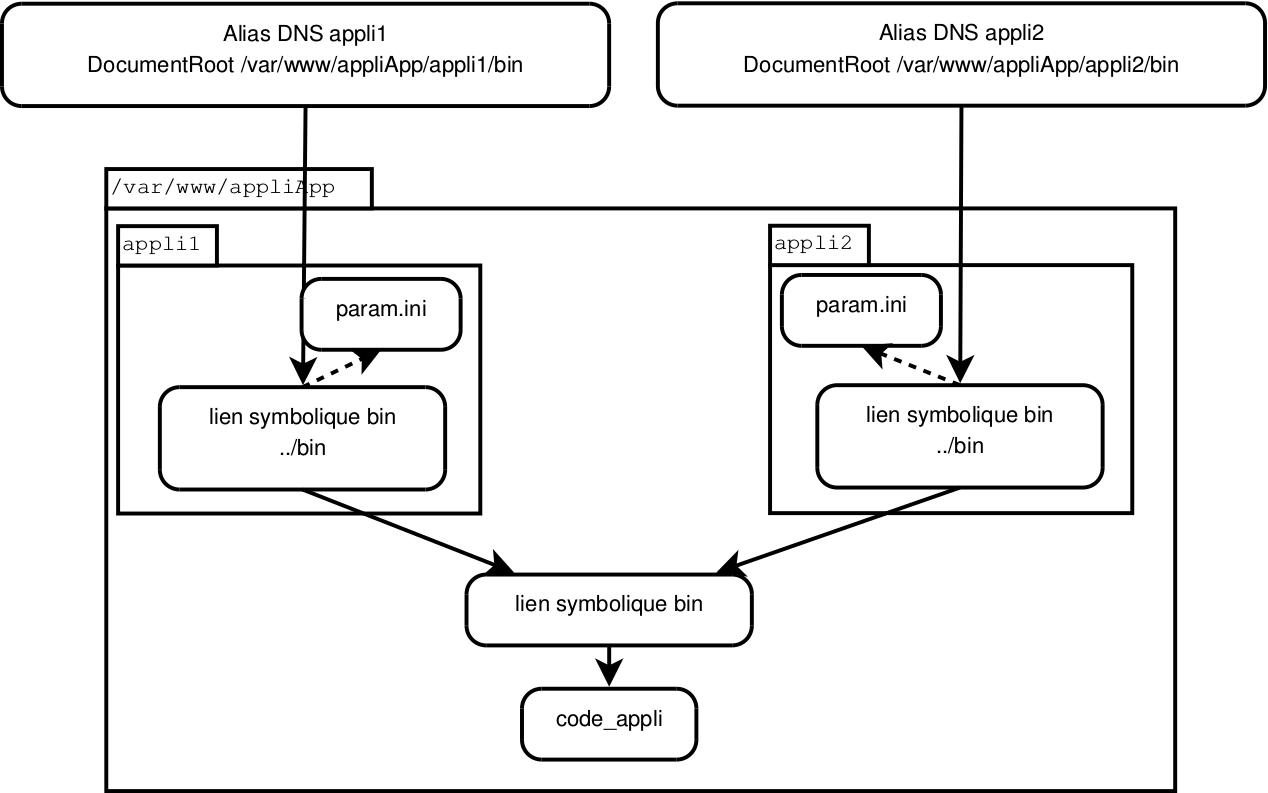
\includegraphics[width=\linewidth]{images/dnsmultiple}
\caption{\label{dnsmultipleschema}Schéma général d’implémentation pour utiliser le même code avec des noms d’application et des jeux de données différents}
\end{figure}

Dans le paramétrage de l’alias DNS (en principe, dans \textit{/etc/apache2/sites-available}), l’application pointe vers le dossier \textit{/var/www/appliApp/appli1/bin}. \textit{/var/www} correspond à la racine du site web, \textit{appliApp} au dossier racine de l’application, \textit{appli1} au dossier spécifique de l’alias DNS. Ce dossier \textit{appli1} ne contient que deux fichiers : \textit{param.ini}, qui contient les paramètres spécifiques, et \textit{bin}, qui est un lien symbolique vers le dossier \textit{../bin}.

Le dossier \textit{../bin} (donc, dans\textit{ /var/www/appliApp}) est lui aussi un alias qui pointe vers le code réel de l’application, ici \textit{code\_appli}. Le fichier \textit{param.inc.php} doit contenir les commandes suivantes pour que le fichier \textit{param.ini} soit correctement chargé selon le contexte :
\begin{lstlisting}
$chemin = substr($_SERVER["DOCUMENT_ROOT"],0, strpos($_SERVER["DOCUMENT_ROOT"],"/bin"));
$paramIniFile = "$chemin/param.ini";
\end{lstlisting}

Le fichier \textit{param.ini} sera cherché dans le dossier parent du code de l’application, c’est à dire soit dans \textit{appli1}, soit dans \textit{appli2} dans cet exemple. Il suffit qu’il contienne les paramètres adéquats pour rendre l’application utilisable dans des contextes différents à partir du même code initial.

Le fichier \textit{param.ini} est le dernier qui est traité par l'application pour récupérer les paramètres. Ceux-ci sont lus dans l'ordre suivant :

\textbf{param/param.default.inc.php $\rightarrow$ param/param.inc.php $\rightarrow$ ../param.ini}

\textit{param.ini} contiendra les entrées spécifiques liées au DNS utilisé pour accéder à l'application, en principe tout ou partie de celles-ci :
\begin{lstlisting}
APPLI_titre="Gestion des collections d'EABX"
BDD_schema=col, public, gacl
BDD_login=compte_de_connexion
BDD_passwd=mot_de_passe_de_connexion
BDD_dsn=pgsql:host=serveur;dbname=base_de_donnees;sslmode=require
GACL_aco=col
APPLI_code=proto
\end{lstlisting}

Si un libellé contient une apostrophe, la chaîne doit être insérée dans des guillemets doubles, comme ici pour la variable \textit{APPLI\_titre}.


\subsection{Droits à attribuer au serveur web}
\label{droitsApache}
Le serveur web doit pouvoir accéder en lecture à l'ensemble des fichiers de l'application, et en écriture à deux dossiers :
\begin{itemize}
\item \textit{display/templates\_c} : fichier utilisé par Smarty pour compiler les modèles de documents HTML ;
\item \textit{temp} : dossier de génération des images et des fichiers temporaires.
\end{itemize}

Deux scripts sont fournis pour attribuer les droits : 
\begin{itemize}
\item \textbf{install/apache2/upgrade\_rights.sh} : positionne les droits en utilisant les droits standards Linux (owner, group)
\item \textbf{install/apache2/upgrade\_rights\_with\_acl.sh} : positionne les droits à partir des ACL.
\end{itemize}

Les scripts doivent être lancés ainsi :
\begin{lstlisting}
collec-2.0/install/apache2/upgrade_rights.sh collec-2.0
\end{lstlisting}
ou 
\begin{lstlisting}
collec-2.0/install/apache2/upgrade_rights_with_acl.sh collec-2.0
\end{lstlisting}


\section{Configurer l'application}

L'application est configurable par l'intermédiaire de trois fichiers :

\textbf{param/param.default.inc.php $\rightarrow$ param/param.inc.php $\rightarrow$ ../param.ini}

Le premier fichier contient les paramètres par défaut. Il est systématiquement fourni à chaque nouvelle version de l'application.

Le second est spécifique de l'implémentation. Il comprend notamment les informations liées à la connexion à la base de données, à la méthode d'identification, ou à la recherche des attributs dans l'annuaire LDAP. 

le troisième est destiné à offrir la possibilité d'accéder, à partir du même code applicatif, à plusieurs bases de données différentes (\textit{cf.} \ref{dnsmultiple} \textit{\nameref{dnsmultiple}}, page \pageref{dnsmultiple}).

Voici les principaux paramètres utilisés :

\subsection{Connexion à la base de données}

Dans la pratique, deux connexions sont nécessaires : l'une pour accéder à la base des droits, l'autre aux données proprement dites. Voici les paramètres à définir :

\begin{longtable}{|p{4cm}|p{11cm}|}
\hline
\textbf{Variable} & \textbf{Signification} \\
\hline
\endhead
BDD\_login & compte de connexion à la base de données \\
\hline
BDD\_passwd & mot de passe associé\\
\hline
BDD\_dsn & adresse de la base de données sous forme normalisée\\
\hline
BDD\_schema & schéma utilisé (plusieurs schémas peuvent être décrits, en les séparant par une virgule - fonctionnement propre à Postgresql)\\
\hline
GACL\_dblogin & compte de connexion à la base de données des droits\\
\hline
GACL\_dbpasswd & mot de passe associé\\
\hline
GACL\_dsn & adresse normalisée \\
\hline
GACL\_schema & schéma utilisé\\
\hline
GACL\_aco & nom du code de l'application utilisé dans la gestion des droits\\
\hline
\caption{Variables utilisées pour paramétrer les connexions}
\end{longtable}

\subsection{Identification des utilisateurs}

\begin{longtable}{|p{6cm}|p{10cm}|}
\hline
\textbf{Variable} & \textbf{Signification} \\
\hline
\endhead
ident\_type & Type d'identification supporté :
\begin{itemize}
	\item BDD : uniquement en base de données
	\item LDAP : uniquement à partir d'un annuaire LDAP
	\item LDAP-BDD : test de connexion d'abord auprès de l'annuaire LDAP, puis en base de données en cas d'échec
	\item CAS : identification auprès d'un serveur CAS (Common Access Service)
	\item CAS-BDD : identification soit interne (par base de données), soit appel par un bouton vers le serveur CAS
	\item HEADER : identification auprès d'une fédération d'identités, comme EDUGAIN. Nécessite un paramétrage particulier du serveur Apache2 (\textit{cf.} \ref{mellon})
\end{itemize}
\\
\hline
CAS\_plugin & Nom du plugin utilisé pour une connexion CAS \\
\hline
CAS\_address & Adresse du serveur CAS, sous la forme : \textit{serveurcas.societe.com} (sans préfixer avec https://)\\
\hline
CAS\_uri="/cas" & chemin interne au serveur CAS pour accéder à l'identification \\
\hline
CAS\_port = 443 & port utilisé pour atteindre le serveur CAS (port https)\\
\hline
CAS\_debug = false & true ou false, pour activer ou non l'enregistrement des fonctions de débogage. À positionner systématiquement à \textit{false} en production \\
\hline
CAS\_CApath = "" & Chemin d'accès au certificat de l'autorité de certification qui correspond au certificat fourni par le serveur CAS (connexion https). Si la chaîne est vide, le certificat n'est pas vérifié. Le chemin doit être renseigné en production \\
\hline
CAS\_get\_groups = 1 & Récupère les groupes fournis par le serveur CAS \\
\hline
CAS\_group\_attribute = "supannEntiteAffectation" & Attribut multivalué contenant la liste des groupes de l'utilisateur, fourni par le serveur CAS \\
\hline
LDAP & tableau contenant tous les paramètres nécessaires pour une identification LDAP \\
\hline
privateKey & clé privée utilisée pour générer les jetons d'identification (ré-identification automatique après une première connexion) \\
\hline
pubKey & clé publique utilisée pour générer les jetons d'identification \\
\hline
tokenIdentityValidity & durée de validité, en secondes, des jetons d'identification\\
\hline
MAIL\_enabled & Si à 1, l'envoi de mail est géré par l'application \\
\hline
CONNEXION\_max\_attemps & nombre maximum d'essais de connexion avant blocage temporaire du compte \\
\hline
CONNEXION\_blocking\_duration & durée de blocage du compte \\
\hline
APPLI\_mailToAdminPeriod & intervalle de temps entre l'envoi d'un mail de notification de blocage de compte à un administrateur \\
\hline
APPLI\_admin\_ttl & durée de vie d'une session d'administration (temps maximum entre deux accès à une page d'administration avant réidentification) \\
\hline
APPLI\_lostPassword & Si à 1, autorise la récupération du mot de passe perdu, par envoi d'un mail avec un lien chiffré. Nécessite également que MAIL\_enabled soit positionné à 1 \\
\hline
ident\_header\_vars & tableau de configuration de l'identification en mode header
\begin{itemize}
	\item radical : racine des libellés des variables
	\item login : champ renvoyé contenant le login (par défaut, le mail)
	\item mail : champ contenant le mail
	\item cn : common name : nom et prénom
	\item organization : nom de l'organisation d'appartenance
	\item organizationGranted : tableau contenant la liste des organisations autorisées
\end{itemize}
\\
\hline

\caption{Variables utilisées pour paramétrer l'identification}
\end{longtable}

\subsubsection{Ré-identification par jeton}

L'application permet de conserver l'identification plus longtemps que celle définie dans le serveur, en rejouant la connexion avec un jeton d'identification chiffré. Cela évite, par exemple, de devoir se ré-identifier toutes les heures si on accède au logiciel à partir d'un terminal mobile (smartphone ou tablette, par exemple).

Les trois dernières variables permettent de configurer ce mode d'identification. 

Le framework peut générer un jeton chiffré après la première identification, qui sera analysé pour savoir si l'utilisateur peut être ré-identifié automatiquement.

Pour que ce mécanisme fonctionne, il faut :
\begin{itemize}
\item que le paramètre \textit{tokenIdentityValidity} ait une durée de validité supérieure à la durée de vie de la session. Il est raisonnable de ne pas fixer une durée de vie supérieure à une journée de travail (10 heures). Le cookie transmis est protégé ;
\item que les clés privée et publique, utilisées pour le chiffrement du jeton, soient accessibles au serveur web (variables \textit{privateKey} et \textit{publicKey}).
\end{itemize}

Le jeton est chiffré avec la clé privée, ce qui lui permet d'être lu, le cas échéant, par l'application. Il contient le login et la date d'expiration. 

Si l'utilisateur déclenche une déconnexion, le jeton est supprimé.

Pour plus d'informations, consultez comment fonctionne le mécanisme de ré-identification par jeton \cite{token}.

\subsection{Configurer l'accès à l'annuaire LDAP}

Les paramètres LDAP sont stockés dans un tableau :
\begin{lstlisting}
$LDAP = array(
		"address"=>"localhost",
		"port" => 389,
		"rdn" => "cn=manager,dc=example,dc=com",
		"basedn" => "ou=people,ou=example,o=societe,c=fr",
		"user_attrib" => "uid",
		"v3" => true,
		"tls" => false,
		"groupSupport"=>true,
		"groupAttrib"=>"supannentiteaffectation",
		"commonNameAttrib"=>"displayname",
		"mailAttrib"=>"mail",
		'attributgroupname' => "cn",
		'attributloginname' => "memberuid",
		'basedngroup' => 'ou=example,o=societe,c=fr'
);
\end{lstlisting}


L'application peut non seulement identifier les utilisateurs auprès de l'annuaire LDAP, mais également récupérer les groupes auxquels ils appartiennent dans celui-ci.

Voici les paramètres à indiquer dans ce cas de figure (valable en principe pour tout annuaire compatible OpenLdap) : 
\begin{longtable}{|p{4cm}|p{11cm}|}
\hline
\textbf{Variable} & \textbf{Signification} \\
\hline
\endhead
address &  adresse de l'annuaire\\
\hline
port & 389 en mode non chiffré, 636 en mode chiffré\\
\hline
rdn & compte de connexion, si nécessaire \\
\hline
basedn & base de recherche des utilisateurs\\
\hline
user\_attrib & nom du champ contenant le login à tester\\
\hline
v3 & toujours à \textit{true}\\
\hline
tls & \textit{true} en mode chiffré\\
\hline
groupSupport & \textbf{true} si l'application recherche les groupes d'appartenance du login dans l'annuaire\\
\hline
groupAttrib & Nom de l'attribut contenant la liste des groupes d'appartenance\\
\hline
commonNameAttrib & Nom de l'attribut contenant le nom de l'utilisateur\\
\hline
mailAttrib & Nom de l'attribut contenant l'adresse mail de l'utilisateur\\
\hline
attributgroupname & Attribut contenant le nom du groupe lors de la recherche des groupes (cn par défaut)\\
\hline
attributloginname & attribut contenant les membres d'un groupe\\
\hline
basedngroup & base de recherche des groupes \\
\hline
\caption{Variables utilisées pour paramétrer l'accès à l'annuaire LDAP}
\end{longtable}

\subsection{Paramètres spécifiques}
\label{paramspec}

\begin{longtable}{|p{4cm}|p{11cm}|}
\hline
\textbf{Variable} & \textbf{Signification} \\
\hline
\endhead
GACL\_aco & nom du code de l'application utilisé dans la gestion des droits (\textit{cf.} section \ref{droits})\\
\hline
APPLI\_code & obsolète. Voir la section \ref{paramdb} \\
\hline
APPLI\_print\_direct \_command & Commande utilisée pour l'impression directe (depuis le serveur des étiquettes). Par défaut, \textit{lpr}, mais \textit{lp} peut être utilisé pour les Raspberry. \\
\hline
APPLI\_max\_file\_size = 10 & Taille maxi en MB des fichiers téléchargés \\
\hline

\caption{Variables spécifiques}
\end{longtable}

\subsection{Paramètres stockés en base de données}
\label{paramdb}

À partir de la version 1.2, certains paramètres peuvent être stockés dans la base de données, pour éviter qu'ils ne soient dépendants de la configuration du serveur.

Ces paramètres sont accessibles depuis le menu \textit{administration}, item \textit{Paramètres de l'application}.

Voici la liste des paramètres actuellement décrits :
\begin{longtable}{|p{4cm}|p{11cm}|}
\hline
\textbf{Variable} & \textbf{Signification} \\
\hline
\endhead
APPLI\_code & Code interne de l'application. \textbf{Ce code est essentiel} : il sera inscrit dans les codes-barres générés, pour s'assurer qu'un échantillon est bien issu de l'application (couple logiciel $\leftrightarrow$ base de données) concernée. Il ne doit pas être modifié après avoir été attribué\\
\hline
APPLI\_title & Titre de l'application, affiché dans le menu \\
\hline
mapDefaultX & Longitude de positionnement du centre de la carte par défaut \\
\hline
mapDefaultY & Latitude de positionnement du centre de la carte par défaut \\
\hline
mapDefaultZoom & facteur de zoom par défaut lors de l'affichage d'une carte \\
\hline
otp\_issuer & Nom de l'application qui est utilisé dans le mécanisme de double-identification (TOTP) \\
\hline
\caption{Paramètres stockés dans la base de données}
\end{longtable}


\section{Créer la base de données}

La base de données est composée de deux schémas : l'un pour stocker les informations d'identification, les droits d'accès et les traces, l'autre pour les données proprement dites.

Le schéma \textit{public} ne devrait jamais être utilisé pour stocker l'information : réservez-le pour les composants communs, comme Postgis.

Les tables de gestion des droits peuvent être communes à plusieurs jeux / applications différentes : la variable \textit{GACL\_aco} permet de séparer la gestion des droits pour chaque application, tout en travaillant à partir des mêmes utilisateurs (répartis le cas échéant dans des groupes différents selon le jeu de données considéré).

Les scripts de création des schémas dans la base de données sont stockés dans le dossier \textit{install/pgsql}. 

\subsection{Créer la base de données et ajouter les extensions}
La base de données doit être créée avec le superutilisateur postgres. Le script \textit{install/init\_by\_psql.sql} permet de réaliser les opérations suivantes :
\begin{itemize}
	\item création du login postgresql \textit{collec}
	\item création de la base de données collec
	\item ajout des extensions nécessaires (deux concernent la création des index, une pour les données géographiques, et la dernière pour implémenter les fonctions cryptographiques)
	\item connexion avec le login \textit{collec} à la base de données \textit{collec}
	\item exécution du script de création des schémas et des tables
\end{itemize}

Ce script peut être exécuté ainsi :
\begin{lstlisting}
cd install
su postgres -c "psql -f init_by_psql.sql"
\end{lstlisting}

Si la base de données est hébergée dans un serveur différent du serveur web, il faut paramétrer auparavant Postgresql pour autoriser la connexion avec le login \textit{collec} depuis le serveur web, en modifiant le fichier /etc/postgresql/11/main/pg\_hba.conf :
\begin{lstlisting}
host collec collec adresse_serveur/32 md5 
\end{lstlisting}
Le premier \textit{collec} correspond au nom de la base de données, le second au login autorisé depuis l'adresse indiquée.

La configuration de Postgresql doit être rechargée :
\begin{lstlisting}
systemctl reload postgresql
\end{lstlisting}

\subsection{Compte par défaut}
Le script crée un compte d'administration par défaut :
\begin{itemize}
\item login : \textbf{admin}
\item mot de passe : \textbf{password}
\end{itemize}

Il devra être supprimé quand un autre compte d'administration aura été créé.

\subsection{Scripts de modification}

Lors de la livraison de nouvelles versions, il est possible que des scripts de modification soient livrés pour mettre à niveau la base de données. Ces scripts doivent être exécutés dans tous les schémas contenant des données applicatives (pour plus de détails, consultez ci-après \textit{\nameref{newVersion}}).

\section{Mise en production}

Une fois l'application configurée, et après avoir créé un nouveau compte d'administration :
\begin{itemize}
\item supprimez le compte \textit{admin}, livré par défaut, qui ne doit pas être conservé. Sa désactivation n'est pas suffisante : si pour une raison ou pour une autre le compte est réactivé, n'importe qui pourra récupérer les droits totaux ;
\item supprimez le dossier \textit{install} qui contient les scripts de création des tables ;
\item déplacez le dossier \textit{database}, qui contient la documentation d'installation et de configuration (elle n'a pas à rester accessible depuis le site web) ;
\item faites une revue des droits, pour vous assurer que tout est correctement configuré.
\end{itemize}

Vous pouvez également tester si la configuration du serveur est correcte en recourant à \textit{ZAProxy} \cite{zaproxy}, qui analysera la communication entre le serveur et un navigateur et identifiera les problèmes éventuels de non conformité (mauvaise réécriture des entêtes HTML suite à une mauvaise configuration du serveur Apache, par exemple).

\section{Installer une nouvelle version}
\label{newVersion}
\subsection{Faites une sauvegarde de la base de données}
Il arrive fréquemment que la structure de la base de données évolue. Avant toute opération, assurez-vous de disposer d'une sauvegarde, dans un autre support.

Un programme de sauvegarde est disponible dans \textit{install/pgsql/backup.sh}. Vous pouvez l'exécuter manuellement ainsi :
\begin{lstlisting}
su postgres -c "install/pgsql/backup.sh"
\end{lstlisting}

La sauvegarde sera stockée dans \textbf{/var/lib/postgresql/backup}.

Si vous avez utilisé le script d'installation automatique, le programme est également présent dans \textit{/var/lib/postgresql}.

\subsection{Sauvegarder le fichier contenant les paramètres de l'application}

Le fichier \textit{param/param.inc.php} contient vos paramétrages spécifiques. Lors de l'installation d'une nouvelle version, il va être supprimé.

Faites-en une copie, et remettez-le en place après avoir installé la nouvelle version.

\subsection{Consultez le fichier news.txt}

Le fichier \textit{param/news.txt} contient la description des modifications apportées au logiciel. Il précise notamment si une mise à jour de la base de données doit être appliquée.

\subsection{Mise à jour de la structure de la base de données}

Le dossier \textit{install/pgsql} contient les scripts de création et de mise à jour de la base de données. Les scripts de mise à jour sont nommés ainsi :
\begin{lstlisting}
col_alter_versionAnterieure-versionMiseAJour.sql
\end{lstlisting}

\textit{versionAnterieure} correspond à la version la plus ancienne qui doit être mise à jour, \textit{versionMiseAJour} la version cible. Par exemple :
\begin{lstlisting}
col_alter_1.2-1.2.3.sql
\end{lstlisting}
indique que toutes les versions entre \textit{1.2} et \textit{1.2.3} doivent être mises à jour avec le script indiqué. Si vous avez \og sauté \fg{} certaines versions du logiciel, il est possible que plusieurs scripts doivent être appliqués.

La mise à jour doit être appliquée dans tous les schémas contenant des données, notamment dans le cas où le même logiciel est utilisé pour gérer plusieurs jeux de données.

Avant d'exécuter les scripts, vérifiez leur contenu, et notamment le nom des schémas.

Ne relancez jamais l'exécution d'un script.

\subsection{Reconfigurer les droits d'accès au serveur web}

Après installation de la nouvelle version du code, n'oubliez-pas de reconfigurer les accès en lecture pour le compte utilisé pour faire fonctionner le serveur web, et en écriture pour les dossiers \textit{temp} et \textit{display/templates\_c} (\textit{cf.} \ref{droitsApache} \textit{\nameref{droitsApache}}, page \pageref{droitsApache}).

\subsection{Supprimer les dossiers inutiles}
Une fois la mise en production validée, supprimez les dossiers \textit{install} et \textit{database}, et faites une revue des droits pour vous assurer qu'il n'y a pas eu de modification intempestive ou que la configuration est toujours correcte.

\subsection{Vérifier la configuration du chiffrement}
Avec un navigateur récent, ou en testant le site (s'il est accessible depuis internet) à partir de \href{https://www.ssllabs.com/ssltest/}{SSLLABS}, vérifiez que l'application soit correctement configurée, notamment au niveau du serveur Apache.

\chapter{Administrer l'application}

\section{Gérer les droits}
\label{droits}

Depuis la version 1.1, les scripts de création des bases de données intègrent la génération initiale des groupes et des droits associés, ceci afin de faciliter la phase de mise en route.

Toutefois, vous devrez créer des groupes d'utilisateurs correspondant à vos projets, et modifier ensuite les projets pour donner les droits adéquats aux groupes créés (\textit{cf.} \ref{projet}, page \pageref{projet}).

\subsection{Principe général}

Les droits sont gérés selon le principe initialement utilisé dans la bibliothèque PHPGACL \cite{phpgacl}, aujourd'hui obsolète. 

Les logins sont déclarés dans des groupes organisés de manière hiérarchique : un groupe hérite des droits attribués à ses parents.

Les droits utilisés dans le logiciel sont associés à des groupes. Il est possible d'attribuer plusieurs droits à un même groupe, et un droit peut être détenu par des groupes différents.

Si le paramètre \textit{\$LDAP["groupSupport"]} est positionné à \textit{true}, les groupes dont fait partie le compte LDAP sont également récupérés. Si ces groupes se voient attribués des droits, les comptes associés les récupéreront automatiquement.

Voici le schéma des tables utilisées pour gérer les droits :

\begin{figure}[H]
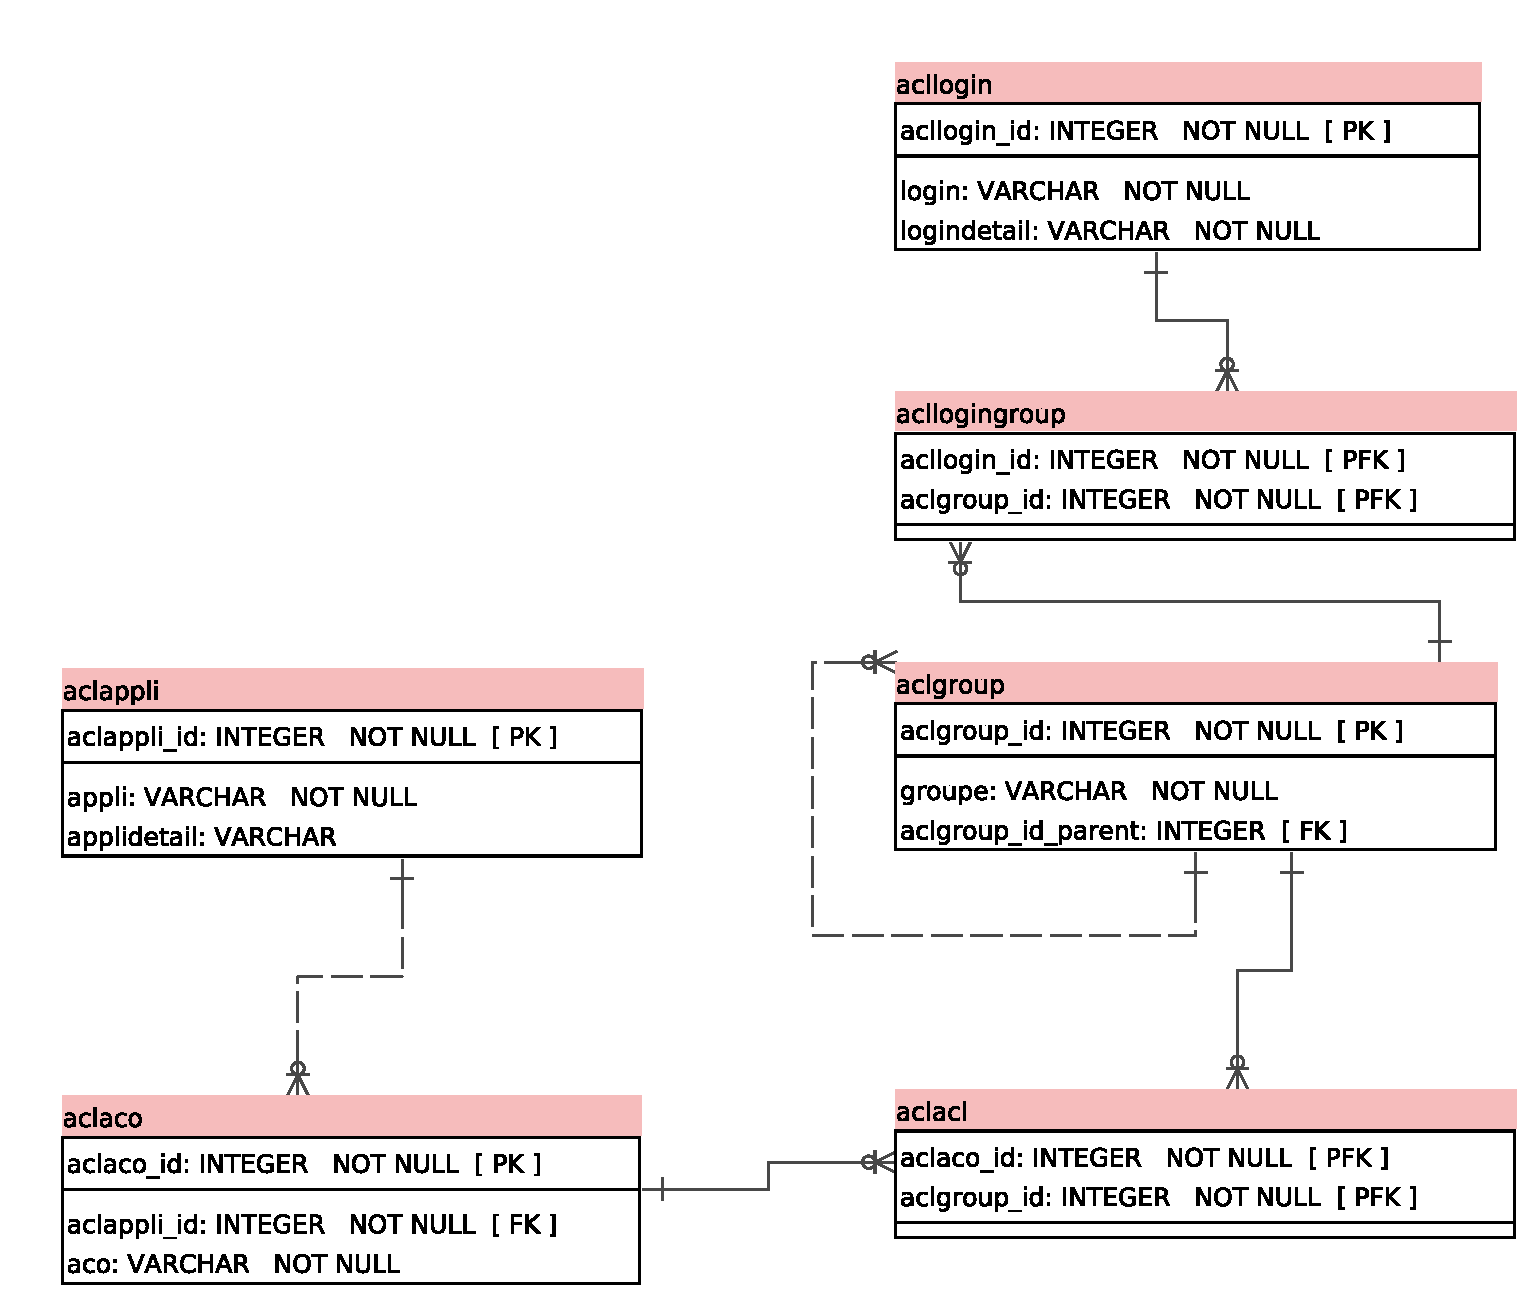
\includegraphics[width=\linewidth]{images/acl_only}
\caption{Schéma des tables utilisées pour gérer les droits}
\end{figure}

Voici la description des tables :
\begin{description}
\item[acllogin] : liste des logins utilisés. Si un compte est créé dans la base locale d'identification, un enregistrement est également créé dans cette table. Pour les identifications LDAP ou CAS, ils doivent être identiques. Si seuls les groupes LDAP sont utilisés pour un compte, il n'a pas besoin d'être décrit ici ;
\item[aclappli] : liste des applications gérées. Il est possible de gérer, à partir de la même base de données, plusieurs ensembles de droits, qui utilisent les mêmes logins.
\item[aclaco] : liste des droits déclarés dans l'application ;
\item[aclgroup] : liste des groupes contenant les logins, et qui détiennent les droits. Un groupe peut hériter d'un autre groupe. Les droits associés au groupe parent sont également attribués au groupe hérité ;
\item[acllogingroup] : table permettant de déclarer les logins associés à un groupe ;
\item[aclacl] : table décrivant les droits détenus par un groupe.
\end{description}

Le module d'administration permet de saisir toutes ces informations. Il faut que l'utilisateur dispose du droit \textit{admin}, c'est à dire qu'il fasse partie du groupe \textit{admin} (configuration par défaut à l'initialisation de la base des droits) pour pouvoir accéder à ces fonctions.

\subsection{Créer un nouvel utilisateur}

Les utilisateurs peuvent être issus soit de l'annuaire LDAP, soit d'un serveur CAS, soit d'un serveur de fédération, soit de la base interne. 
Pour créer un nouvel utilisateur dans la base locale :
\begin{itemize}
\item \textit{Administration $\rightarrow$ Liste des comptes }
\item \textit{Nouveau login}
\item renseignez au minimum le login.
\end{itemize}

\begin{figure}[H]
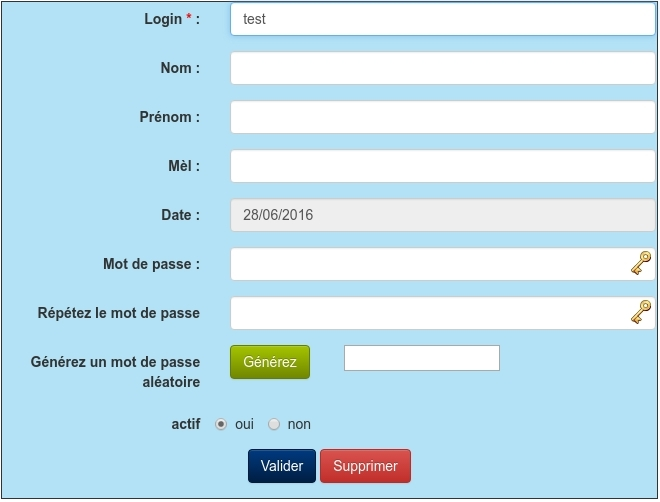
\includegraphics[width=\linewidth]{images/user_create}
\caption{Écran de saisie d'un login de connexion}
\end{figure}

Pour créer le mot de passe, vous pouvez cliquer sur le bouton \textit{Générez}, qui  en générera un automatiquement. Envoyez-le par mél à son destinataire (par \textit{copier-coller}), en lui demandant de le modifier à la première connexion (icône en forme de clé, dans le bandeau, en haut à droite).

Les mots de passe doivent respecter les règles suivantes :
\begin{itemize}
\item ils doivent avoir une longueur minimale de 8 caractères ;
\item ils doivent comprendre trois types de caractères différents parmi les minuscules, majuscules, chiffres et caractères de ponctuation ;
\item ils ne peuvent pas être réutilisés pour le même login ;
\item les mots de passe n'expirent pas.
\end{itemize}

Les mots de passe sont stockés sous forme d'empreinte, calculée en rajoutant un sel\footnote{chaîne de caractère rajoutée au mot de passe -- en général le login ou un identifiant -- qui permet d'éviter que deux mots de passe identiques, associés à deux logins différents, aient la même empreinte} et encodés en SHA256 : ils ne peuvent pas être retrouvés en cas de perte.

La création d'un compte entraîne la création d'une entrée identique dans la table des \textit{acllogin}, utilisée pour attribuer les droits.

Pour désactiver temporairement un compte, sélectionnez \textit{non} dans la zone \textit{actif}. Si le compte ne doit plus être utilisé, supprimez-le.

Attention : si le compte disposait des droits d'administration, assurez-vous que vous avez toujours un compte disposant des mêmes droits avant la suppression.

\subsection{Créer un login utilisé dans la gestion des droits}

Indépendamment du compte de connexion, qui peut être soit issu de la base interne, soit récupéré auprès d'un annuaire LDAP ou d'un serveur CAS, l'application a besoin de connaître les utilisateurs pour pouvoir leur attribuer des droits.

À partir du menu, choisissez \textit{Administration $\rightarrow$ ACL - logins}.

Vous pouvez modifier un login existant ou en créer un nouveau. Dans ce cas, vous devrez indiquer au minimum le login utilisé (identique à celui qui est employé pour la connexion à l'application : base de données interne, annuaire LDAP, serveur CAS).

\begin{figure}[H]
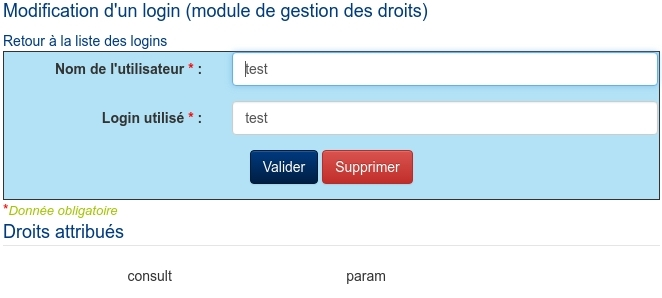
\includegraphics[width=\linewidth]{images/acl_login}
\caption{Écran de modification d'un login dans le module de gestion des droits}
\end{figure}


Sous l'écran de saisie figurent la liste des droits attribués à un login (en modification, le calcul n'est réalisé qu'à l'affichage de la page).

\subsection{Définir les groupes d'utilisateur}

Les groupes d'utilisateurs sont gérés selon un mécanisme d'héritage. Un groupe de haut niveau hérite des groupes précédents : si des droits ont été attribués à un groupe de niveau inférieur, un login associé à un groupe de niveau supérieur les récupère également.

Pour définir les groupes, dans le menu, choisissez \textit{Administration $\rightarrow$ ACL - groupes de logins}.

\begin{figure}[H]
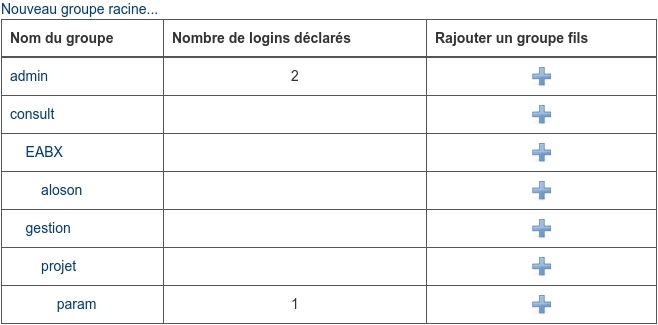
\includegraphics[width=\linewidth]{images/acl_groupe}
\caption{Liste des groupes de logins}
\end{figure}

Ainsi, le login déclaré dans le groupe \textit{param} récupérera les droits attribués aux groupes \textit{projet}, \textit{gestion} et \textit{consult}.

Pour créer un groupe, deux possibilités :
\begin{itemize}
\item soit le groupe est à la base d'une nouvelle branche : utilisez alors \textit{Nouveau groupe racine...} ;
\item soit le groupe hérite d'un autre groupe : cliquez sur le signe + (\textit{Rajouter un groupe fils}).
\end{itemize}

Vous pouvez indiquer les logins qui sont rattachés à ce groupe.


\subsection{Créer une application}
Le moteur utilisé pour faire fonctionner le logiciel COLLEC permet de gérer des droits différents pour des jeux de données différents, à partir du même code applicatif. Chaque couple \textit{logiciel} $\leftrightarrow$ \textit{base de données} constitue donc une \textit{application}, au sens de la gestion des droits.

Il est ainsi possible, à partir de la même base de données, de définir des droits différents selon les jeux de données utilisés (un jeu de données correspond à un schéma de base de données comprenant l'intégralité des tables applicatives).

À partir du menu, choisissez \textit{Administration $\rightarrow$ ACL - droits} :
\begin{figure}[H]
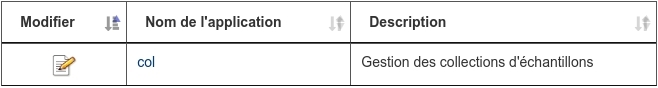
\includegraphics[width=\linewidth]{images/liste_appli}
\caption{Liste des applications déclarées}
\end{figure}

Pour créer une nouvelle application, choisissez \textit{Nouvelle application...}. 

\begin{figure}[H]
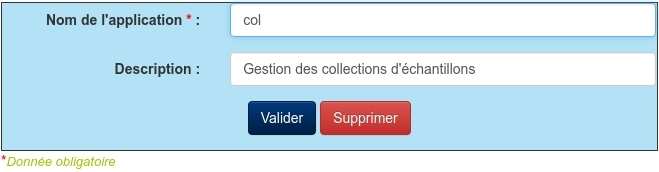
\includegraphics[width=\linewidth]{images/appli_change}
\caption{Écran de saisie d'une application}
\end{figure}

Le nom de l'application doit impérativement correspondre à la valeur \textit{\$GACL\_appli} dans les fichiers de paramètres : c'est ce qui permet au framework de savoir quels droits appliquer.

\subsection{Définir les droits utilisables dans l'application}

À partir de la liste des applications, cliquez sur le nom de celle pour laquelle vous voulez définir les droits utilisables. 
À partir de la liste, sélectionnez \textit{Nouveau droit...}.

\begin{figure}[H]
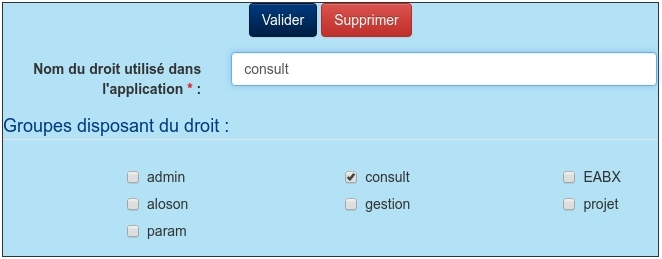
\includegraphics[width=\linewidth]{images/appli_droit}
\caption{Écran de saisie des droits associés à une application}
\label{applidroit}
\end{figure}

Le nom du droit doit être celui défini dans le corps de l'application (les droits sont positionnés dans les fichiers \textit{param/actions.xml}, qui contient la liste des modules utilisables, et \textit{param/menu.xml}, qui sert à générer le menu -- \textit{cf.} table \ref{droitsCollec} \textit{\nameref{droitsCollec}}, page \pageref{droitsCollec}).

Indiquez les groupes d'utilisateurs qui seront associés au droit courant.

\subsection{Cas particulier des groupes et des logins issus d'un annuaire LDAP ou d'un serveur CAS}

Si vous avez paramétré l'application pour qu'elle s'appuie sur un annuaire LDAP pour gérer l'affectation des utilisateurs dans les groupes, ou si vous utilisez un serveur CAS qui fournit également la liste des groupes de l'utilisateur,
vous n'êtes pas obligés de les déclarer explicitement dans le module de gestion des droits.

\subsubsection{Droits attribués à un groupe LDAP ou un groupe CAS}

Tous les utilisateurs d'un groupe héritent d'un droit dans l'application.

\begin{itemize}
\item définissez le nom du groupe (en respectant la casse) dans le tableau des groupes d'utilisateurs (par exemple, EABX) ;
\item sélectionnez le nom de ce groupe dans les droits utilisables ;
\item tous les utilisateurs de l'annuaire LDAP ou du serveur CAS récupéreront automatiquement les droits attribués à ce groupe.
\end{itemize}

\subsubsection{Droits attribués à un utilisateur particulier de l'annuaire LDAP ou du serveur CAS}

Un utilisateur s'identifie auprès de l'annuaire LDAP, mais dispose de droits particuliers.

\begin{itemize}
\item créez son login dans la gestion des droits ;
\item rajoutez-le dans le groupe d'utilisateurs adéquat.
\end{itemize}


\section{Droits spécifiques de l'application COLLEC-SCIENCE}

\subsection{Droits à positionner}
Voici les droits nécessaires pour faire fonctionner correctement l'application :

\begin{longtable}{|p{5cm}|p{10cm}|}
\hline
\textbf{Droit} & \textbf{Usage} \\
\hline
\endhead
admin &	Gestion des utilisateurs et des droits\\
\hline
param &	Définition des tables de paramètres généraux, gestion des collections\\
\hline
collection & rajout des types d'échantillons ou de conteneurs, import de masse \\
\hline
import & permet de réaliser des importations de masse \\
\hline
gestion &	Ajout d'un échantillon pour les projets autorisés, entrée/sortie. Droit attribué par défaut si l'utilisateur fait partie d'au moins un projet \\
\hline
consult	& Consultation des informations, sans possibilité de modification. Le droit de consultation doit être indiqué volontairement\\
\hline

\caption{\label{droitsCollec}Liste des droits utilisés}
\end{longtable}

Ces droits doivent être définis pour chaque application (couple \textit{logiciel} $\leftrightarrow$ \textit{base de données}) gérée par la base de gestion des droits.

\subsection{Gestion des collections}
\label{projet}

Les échantillons étant obligatoirement rattachés à une collcction, vous devrez en créer au minimum une à partir du menu de paramétrage. Un utilisateur avec les droits de gestion ne peut modifier que les échantillons pour lesquels il est autorisé (les collections qui sont rattachées au(x) groupe(s) dont il fait partie).

Voici le principe de gestion des droits pour les collections :
\begin{itemize}
\item Dans \textit{Administration} > \textit{ACL - Groupes de logins}, déclarez les groupes adéquats. En cas d'utilisation des groupes LDAP, les saisir avec la même casse que dans l'annuaire (EABX p. e.).

Il est possible de définir une hiérarchie des groupes, quelle que soit l'origine de l'affectation (base de données ou annuaire Ldap).
Dans le cas où l'annuaire Ldap n'est pas utilisé pour gérer les groupes, renseignez les logins en face des groupes dans le même écran ;
\item Dans les collections, sélectionnez les groupes autorisés (\textit{cf.} \ref{applidroit} \textit{\nameref{applidroit}}, page \pageref{applidroit}) ;
\item les utilisateurs faisant partie des groupes autorisés disposeront des droits de \textit{gestion} pour la collection considérée.
\end{itemize}

\section{Configurer les paramètres généraux}
\label{param}
L'ensemble des paramètres sont accessibles à partir du menu \textit{Paramètres}. 

Par défaut, tous les utilisateurs qui disposent du droit de consultation peuvent visualiser les paramètres. La modification n'est possible que pour ceux qui disposent des droits suivants :

\begin{longtable}{|p{4cm}|p{8cm}| p{3cm}|}
\hline
\textbf{Nom} & \textbf{Description} & \textbf{Droit nécessaire} \\
\hline
\endhead
Projets & Liste des projets et droits associés & admin \\
\hline
Protocoles & Protocoles de prélèvement des échantillons & collection \\
\hline
Opérations & Opérations rattachées aux protocoles & collection \\
\hline
Type d'événement & Événements survenant aux objets & param \\
\hline
Familles de conteneurs & Mécanisme pour retrouver les conteneurs selon leur nature (pièce, caisse...) & param, projet\\
\hline
Conditions de stockage & Mécanisme de conservation (lyophilisation, p. e.) & param, collection\\
\hline
Motifs de déstockage & Raisons invoquées pour sortir un objet du stock & param, collection\\
\hline
Types de conteneurs & Modèles de conteneurs (porteurs des étiquettes, entre autres) & param, collection\\
\hline
Statut des objets & Liste des statuts que peut prendre un objet & param\\
\hline
Type d'échantillon & Modèles des échantillons (rattachables à un type de conteneur) &  param, collection\\
\hline
Sous-échantillonnage & Pour les échantillons composés d'éléments non différenciables, unité utilisée pour réaliser le sous-échantillonnage (nombre, volume...) & param \\
\hline
Étiquettes & Modèles des étiquettes imprimables & param \\
\hline
Types d'identifiants & Types d'identifiants complémentaires des objets & param \\
\hline

\caption{Liste des paramètres et droits de modification associés}
\end{longtable}

\section{Créer ou modifier un modèle d'étiquettes}

\begin{figure}[H]
\centering
\fbox{
\includegraphics{images/etiquette}}
\caption{Exemple d'étiquette}
\end{figure}

Les étiquettes sont créées en recourant au logiciel FOP \cite{fop}, écrit en Java. Voici les opérations réalisées par l'application pour générer les étiquettes :
\begin{itemize}
\item pour chaque objet concerné (des containers ou des échantillons associés à un type de container, et si le type de container est rattaché à un modèle d'étiquettes), une image du QRcode est générée dans le dossier \textit{temp} ;
\item dans le dossier \textit{temp}, un fichier au format XML est généré, contenant les informations à imprimer sur l'étiquette ;
\item un fichier au format XSL, qui contient les ordres de création de l'étiquette, est également créé dans le même dossier. Le contenu de ce fichier est issu d'un enregistrement provenant de la table \textit{label} ;
\item le programme PHP fait appel à FOP pour générer, à partir du fichier XML et en utilisant le fichier XSL, un fichier PDF. Une page du fichier correspond à une étiquette (mécanisme utilisé par les imprimantes à étiquettes pour les séparer).
\end{itemize}

La configuration du modèle d'étiquettes revient à définir à la fois le contenu des informations qui seront insérées dans le QRCODE et la forme que prendra l'étiquette, c'est à dire les informations qui seront imprimées, le format, etc. Cette forme reprend la syntaxe XSL comprise par FOP.

\begin{figure}[H]
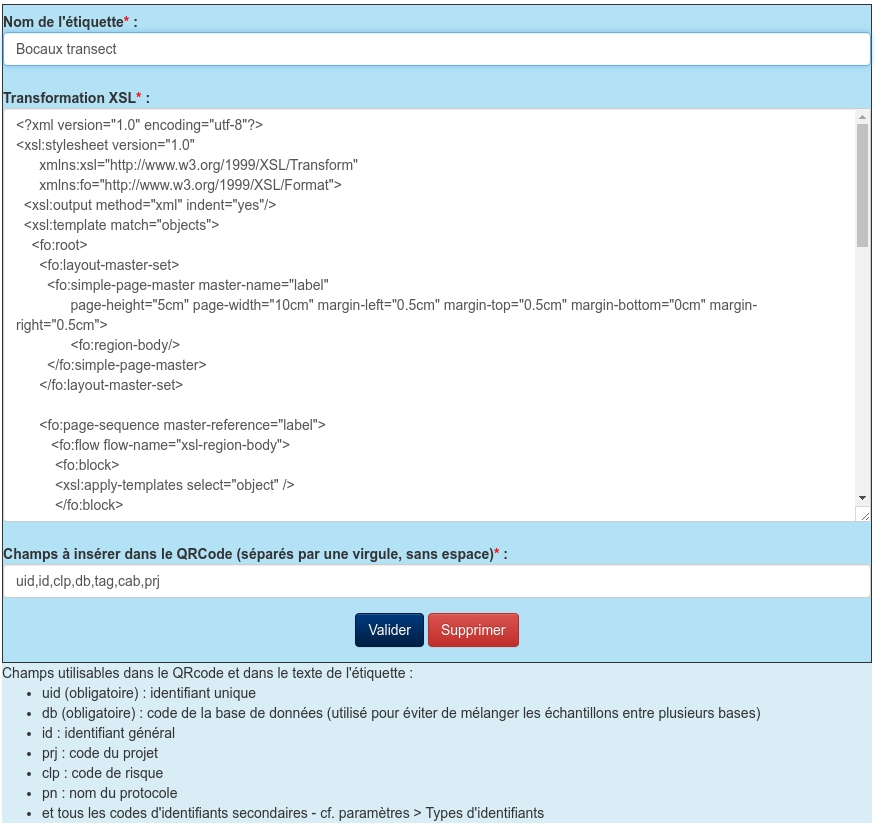
\includegraphics[width=\linewidth]{images/label}
\caption{Écran de saisie d'un modèle d'étiquette}
\end{figure}

\subsection{Définir le contenu du QRcode}
Le QRcode est un format de code barre normalisé en deux dimensions, qui permet de stocker jusqu'à 2000 caractères en 8 bits. 

Le principe retenu dans l'application est de stocker l'information au format JSON. Pour limiter la taille du code barre, les noms des balises doivent être les plus petites possibles. Voici les balises obligatoires à insérer systématiquement dans une étiquette :

\begin{longtable}{|p{3cm}|p{12cm}| }
\hline
\textbf{Nom} & \textbf{Description} \\
\hline
\endhead
uid & Identifiant unique de l'objet dans la base de données \\
\hline
db & Identifiant de la base de données. C'est la valeur du paramètre \textit{APPLI\_code} (\textit{cf.} \ref{paramspec} \textit{\nameref{paramspec}}, page \pageref{paramspec}) \\
\hline
\caption{Liste des balises à insérer obligatoirement dans les QRcodes}
\end{longtable}

D'autres informations peuvent être également insérées :
\begin{longtable}{|p{3cm}|p{12cm}| }
\hline
\textbf{Nom} & \textbf{Description} \\
\hline
\endhead
id & Identifiant métier principal (champ \textit{identifiant ou nom}, en saisie) \\
\hline
prj & Code de la collection (pour les échantillons) \\
\hline
clp & Code du risque associé au conteneur, en raison du produit de conservation utilisé \\
\hline
pn & Nom du protocole de collecte des échantillons \\
\hline
autres codes & tous les codes d'identification secondaires définis dans la table de paramètres \textit{Types d'identifiants} (\textit{cf.} \ref{param} \textit{\nameref{param}}, page \pageref{param}). \\
\hline
les champs utilisés dans les métadonnnées & les codes des champs utilisés dans la description des métadonnées. Un modèle d'étiquette ne peut être associé qu'à un type de métadonnées \\
\hline

\caption{Liste des balises facultatives insérables dans les QRcodes}
\end{longtable}

\subsection{Configuration du fichier XSL}

La syntaxe particulière du fichier XSL ne doit être modifiée qu'en conservant la version initiale (recopie dans un bloc-notes, par exemple), pour éviter de perdre une configuration opérationnelle suite à un mauvais paramétrage.

Voici la description du contenu du fichier et les zones modifiables.

\subsubsection{Entête du fichier}
Elle permet de modifier la taille de l'étiquette (largeur et hauteur maximale). Vous ne devriez changer que les attributs \textit{page-height} et \textit{page-width}. Pour les marges (attributs \textit{margin-}), soyez prudents et vérifiez notamment que les QRcodes ne soient pas rognés à cause de marges insuffisantes.

\begin{lstlisting}
<?xml version="1.0" encoding="utf-8"?>
<xsl:stylesheet version="1.0"
      xmlns:xsl="http://www.w3.org/1999/XSL/Transform"
      xmlns:fo="http://www.w3.org/1999/XSL/Format">
  <xsl:output method="xml" indent="yes"/>
  <xsl:template match="objects">
    <fo:root>
      <fo:layout-master-set>
        <fo:simple-page-master master-name="label"
              page-height="5cm" page-width="10cm" 
              margin-left="0.5cm" 
              margin-top="0.5cm" 
              margin-bottom="0cm" 
              margin-right="0.5cm">  
              <fo:region-body/>
        </fo:simple-page-master>
      </fo:layout-master-set>
      
      <fo:page-sequence master-reference="label">
         <fo:flow flow-name="xsl-region-body">        
          <fo:block>
          <xsl:apply-templates select="object" />
          </fo:block>

        </fo:flow>
      </fo:page-sequence>
    </fo:root>
   </xsl:template>
  <xsl:template match="object">
\end{lstlisting}

\subsubsection{Format de l'étiquette}
Le contenu de l'étiquette est décrit sous la forme d'un tableau (balises \textit{fo:table}). La première colonne contient le QRCode, la seconde le texte associé.

Ici, deux colonnes de taille identique (4 cm chacune) sont définies.

\begin{lstlisting}
  <fo:table table-layout="fixed" border-collapse="collapse"  
  border-style="none" width="8cm" 
  keep-together.within-page="always">
  <fo:table-column column-width="4cm"/>
  <fo:table-column column-width="4cm" />
 <fo:table-body  border-style="none" >
\end{lstlisting}

Les cellules (\textit{table-cell}) sont insérées dans une ligne (\textit{table-row}) :

\begin{lstlisting}
 	<fo:table-row>
\end{lstlisting}

\subsubsection{Insertion du QRcode}
Le QRcode est inséré dans un bloc. Les seules informations modifiables sont celles concernant la hauteur (attribut \textit{height} et la largeur (attribut \textit{content-width})). Veillez à ce que la hauteur et la largeur soient identiques, et ne modifiez pas les autres informations.

\begin{lstlisting}
  		<fo:table-cell> 
  		<fo:block>
  		<fo:external-graphic>
      <xsl:attribute name="src">
             <xsl:value-of select="concat(uid,'.png')" />
       </xsl:attribute>
       <xsl:attribute name="content-height">
       scale-to-fit
       </xsl:attribute>
       <xsl:attribute name="height">4cm</xsl:attribute>
        <xsl:attribute name="content-width">4cm</xsl:attribute>
        <xsl:attribute name="scaling">uniform</xsl:attribute>      
       </fo:external-graphic>
 		</fo:block>
   		</fo:table-cell>
\end{lstlisting}
\subsubsection{Contenu textuel}

Les autres informations sont affichées dans des blocs, avec une ligne par catégorie d'information.

L'étiquette commence ici par indiquer l'établissement (ici, IRSTEA), écrit en gras.

\begin{lstlisting}
  		<fo:table-cell>
		<fo:block>
			<fo:inline font-weight="bold">
				IRSTEA
			</fo:inline>
		</fo:block>
\end{lstlisting}

Chaque information est affichée dans un bloc, comprenant un titre (par exemple, \textit{uid}), associé à une ou plusieurs valeurs. Ainsi, la première ligne affiche sur la même ligne, et en gras (attribut \textit{font-weight="bold"}), le code de la base de données (\textit{<xsl:value-of select="db"/>}) et l'UID de l'objet (\textit{<xsl:value-of select="uid"/>}).

\begin{lstlisting}   		

  			<fo:block>uid:
  			<fo:inline font-weight="bold">
  			<xsl:value-of select="db"/>:
  			<xsl:value-of select="uid"/></fo:inline>
  			</fo:block>
  			<fo:block>id:
  			<fo:inline font-weight="bold"> 
  			<xsl:value-of select="id"/></fo:inline>
  			</fo:block>
  			<fo:block>prj:
  			<fo:inline font-weight="bold"> 
  			<xsl:value-of select="prj"/></fo:inline>
  			</fo:block>
  			<fo:block>clp:
  			<fo:inline font-weight="bold">
  			<xsl:value-of select="clp"/></fo:inline>
  			</fo:block>
\end{lstlisting}

\subsubsection{Fin de l'étiquette}

Une fois toutes les informations affichées, le tableau est fermé, et un saut de page est généré systématiquement :
\begin{lstlisting}
  		</fo:table-cell>
  	  	</fo:table-row>
  </fo:table-body>
  </fo:table>
   <fo:block page-break-after="always"/>
\end{lstlisting}

Enfin, le fichier XSL est correctement fermé :
\begin{lstlisting}
  </xsl:template>
</xsl:stylesheet>
\end{lstlisting}

Il est possible de créer des étiquettes avec des formats différents, par exemple en créant plusieurs lignes. Pensez à fermer vos balises, et qu'elles soient correctement imbriquées, pour éviter tout souci.

Pour aller plus loin dans la mise en page, consultez la documentation du projet FOP.

\section{Gestion des traces}

Tous les appels lancés par les utilisateurs vers les modules de l'application sont enregistrés dans la table \textit{gacl.log}, qui ne doit être accessible qu'aux personnes dûment autorisées. Les traces sont supprimées au bout d'un an (script de nettoyage exécuté lors de la connexion d'un utilisateur).

Voici un exemple de trace générée :
\begin{lstlisting}
log_id	login	nom_module	log_date	commentaire	ipaddress
523437	eric.quinton	col-Sample-write	2016-10-25 14:57:01	16	::1
523438	eric.quinton	col-sampleDisplay	2016-10-25 14:57:01	ok	::1
523436	eric.quinton	col-sampleWrite	2016-10-25 14:57:00	ok	::1
523435	eric.quinton	col-sampleChange	2016-10-25 14:56:58	ok	::1
523434	eric.quinton	col-sampleDisplay	2016-10-25 14:56:55	ok	::1
523433	eric.quinton	col-sampleList	2016-10-25 14:56:52	ok	::1
523431	eric.quinton	col-default	2016-10-25 14:53:05	ok	::1
523430	eric.quinton	col-connexion	2016-10-25 14:53:04	ldap-ok	::1
523429	unknown	col-connexion	2016-10-25 14:52:57	ok	::1
\end{lstlisting}

La colonne \textit{commentaire}, pour la ligne 523437, contient l'identifiant modifié (l'enregistrement 16 a été traité par le module sampleWrite -- Sample (majuscule du S) correspond au nom de la classe qui a été utilisée pour réaliser l'écriture vers la base de données). L'adresse IP est théoriquement celle de l'utilisateur (ici, connexion locale), y compris en prenant en compte le passage par un serveur Reverse-proxy\footnote{serveur mis en entrée du réseau privé, qui permet de masquer les adresses internes et de contrôler les accès depuis Internet}.

Parallèlement, les messages d'erreur sont envoyés au processus Linux SYSLOG, qui enregistre les traces dans le fichier \textit{/var/log/apache2/error.log}.

\chapter{Comment faire pour ?}
\section{Générer une liste d'échantillons vides}
Objectif : préparer des bocaux d'échantillons avant de partir en campagne de collecte. Ces bocaux doivent être étiquetés.

Le logiciel propose une procédure d'import de masse, qui permet de répondre à cette question.

Voici la méthode à utiliser :
\begin{itemize}
\item générez un fichier au format CSV (créé par exemple à partir de LibreOffice OpenDataSheet -- ODS), qui comprend une ligne par échantillon ;
\item lancez la procédure d'import : le programme vous indiquera les UID générés ;
\item recherchez les UID générés, et déclenchez l'impression des étiquettes.
\end{itemize}

\subsection{Structure du fichier CSV}

Toute opération d'import présente des risques : il est difficile de revenir en arrière une fois celle-ci terminée.
Pour les limiter, le logiciel va procéder en deux étapes. D'abord, la structure du fichier va être analysée, et la cohérence des informations indiquées vérifiée.
Ensuite, si aucune anomalie n'est détectée, l'import pourra être déclenché.

La première ligne du fichier doit comporter le nom des colonnes. Leur nom est normalisé et ne doit en aucun cas être modifié. Si une colonne n'existe pas, l'import du fichier sera rejeté.

Les identifiants numériques (\textit{project\_id} par exemple) doivent être recherchés dans les tables de paramètres de l'application.

Voici la liste des colonnes utilisables :
\begin{longtable}{|p{4cm}|p{8cm}| c|}
\hline
\textbf{Colonne} & \textbf{Description} & \textbf{Obligatoire} \\
\hline
\endhead
sample\_identifier & identifiant métier de l'échantillon & X \\
\hline
collection\_id & identifiant de la collection de rattachement & X \\
\hline
sample\_type\_id & identifiant du type d'échantillon & X \\
\hline
sample\_status\_id & identifiant du statut à attribuer & X \\
\hline
sampling\_place\_id & le numéro informatique de l'endroit où l'échantillon a été prélevé & \\
\hline
wgs84\_x & longitude GPS en WGS84 (degrés décimaux) & \\
\hline
wgs84\_y & latitude GPS en WGS84 (degrés décimaux) & \\
\hline
sampling\_date & date de création/échantillonnage de l'échantillon, au format dd/mm/yyyy & \\
\hline
expiration\_date & date d'expiration de l'échantillon, au format dd/mm/yyyy & \\
\hline
sample\_location & emplacement de rangement de l'échantillon dans le container (texte libre) & \\
\hline
sample\_column & n° de la colonne de stockage dans le container & \\
\hline
sample\_line & n° de la ligne de stockage dans le container & \\
\hline
sample\_multiple\_value & le nombre total de sous-échantillons (ou le volume total, ou le pourcentage...) contenu dans l'échantillon si le type d'échantillons utilisé le permet (valeur numérique, séparateur décimal : point) & \\
\hline
sample\_parent\_uid & UID du parent (création d'échantillons rattachés) &\\
\hline
sample\_metadata\_json & métadonnées rattachées à l'échantillon (au format json, p. e. : \{"taxon":"Alosa alosa"\}) & \\
\hline
container\_identifier & identifiant du container & X \\
\hline
container\_type\_id & identifiant du type de container & X \\
\hline
container\_status\_id & identifiant du statut à attribuer au container & \\
\hline
container\_column & n° de la colonne de stockage dans le container parent & \\
\hline
container\_line & n° de la ligne de stockage dans le container parent & \\
\hline
container\_parent\_uid & UID du container dans lequel le container courant est rangé & \\
\hline
identifiants complémentaires & une colonne par code supplémentaire (menu \textit{Paramètres $\rightarrow$ Types d'identifiants}) & \\
\hline

\caption{Liste des colonnes utilisables lors d'un import de masse}
\end{longtable}

Les champs obligatoires ne le sont que si l'identifiant de l'objet considéré -- échantillon ou container -- a été renseigné. Une ligne doit contenir au minimum soit un numéro d'échantillon, soit un numéro de container.

\subsection{Procédure d'import}

À partir du menu, choisissez \textit{Objet $\rightarrow$ import de masse}. Seuls les utilisateurs qui disposent du droit \textit{projet} ou \textit{import} pourront réaliser l'opération.
\begin{figure}[H]
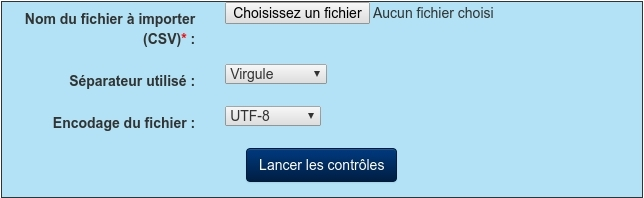
\includegraphics[width=\linewidth]{images/import_controle}
\caption{Sélection du fichier pour un import de masse}
\end{figure}

Sélectionnez le fichier à importer, vérifiez le séparateur utilisé. Préférez, si possible, les données au format UTF-8.

L'import sera réalisé ainsi :
\begin{enumerate}

\item  si sample\_identifier est renseigné : création de l'échantillon
\item    si container\_identifier est renseigné : création du container
\item    si container\_identifier et container\_parent\_uid sont renseignés : création du mouvement d'entrée du container
\item    si l'échantillon et le container ont été créés, création du mouvement d'entrée de l'échantillon dans le container
\item    si l'échantillon est créé, que container\_parent\_uid est renseigné, et que container\_identifier n'est pas rempli, création du mouvement d'entrée de l'échantillon dans le container indiqué

\end{enumerate}

Si des anomalies sont détectées lors du contrôle, un tableau récapitulant les problèmes rencontrés sera affiché, ressemblant à ceci :
\begin{figure}[H]
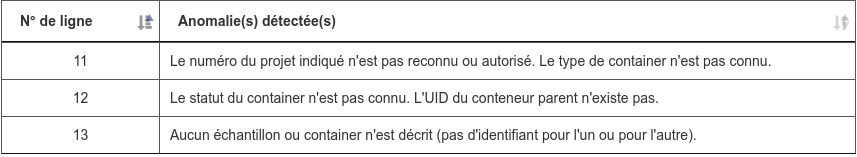
\includegraphics[width=\linewidth]{images/import_tableau}
\caption{Exemples d'anomalies détectées lors du contrôle de l'import}
\end{figure}

Si les contrôles se sont bien déroulés, le programme proposera alors de déclencher l'import, et affichera en retour les valeurs \textit{mini} et \textit{maxi} des UID générées.

\subsection{Autre usage}
Cette fonctionnalité peut également être utilisée pour déclencher l'import de listes d'échantillons pré-existants, et de créer automatiquement les mouvements adéquats pour les ranger dans leurs containers de stockage.

\subsection{Exemple de fichier}
\begin{figure}[H]
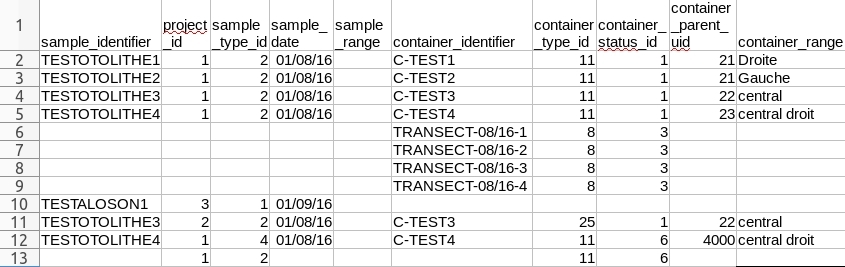
\includegraphics[width=\linewidth]{images/importcsv}
\caption{Exemple d'un fichier CSV}
\end{figure}

Dans cet exemple, l'import ne sera pas réalisé pour les raisons suivantes :
\begin{itemize}
\item en ligne 12, le numéro de container n'existe pas ;
\item la ligne 13 ne contient ni numéro d'échantillon, ni de numéro de container.
\end{itemize}

Sans tenir compte des erreurs, voici les opérations qui seraient exécutées :
\begin{itemize}
\item lignes 2 à 5, 11 et 12 : création d'échantillons, avec création du mouvement d'entrée dans les containers correspondants ;
\item lignes 6 à 9 : création de containers ;
\item ligne 10 : création d'un échantillon non rangé ;
\end{itemize}

\section{Export de données au format JSON}

Il est possible d'exporter un lot de données, réparties sur plusieurs tables, pour les réimporter dans une autre base de données. Par défaut, l'export \og technique\fg{} des modèles d'exports est disponible.

Les données sont exportées au format JSON.

\subsection{Description des modèles d'export}

Choisissez le menu \textit{Paramètres > Modèles d'export}. Hormis le nom du modèle, toutes les autres informations permettent de décrire les tables à exporter et les relations entre elles.

La saisie d'une nouvelle table passe par l'ajout d'un nouvel item dans la partie \textit{Description du modèle}. Chaque item peut être déplacé après création, si nécessaire.

Pour chaque table à exporter, voici les informations à renseigner :
\begin{itemize}
	\item nom de la table, telle qu'il figure dans la base de données
	\item alias de la table : si une même table peut être reliée à des tables parentes différentes, cette colonne devra être renseignée avec un nom différent pour chaque instance. 
	\item  clé primaire : indiquez la clé primaire utilisée dans la table. Elle ne doit pas être renseignée dans le cas d'une table porteuse d'une relation n-n, dont la clé est composée des clés des deux tables parentes.
	\item clé métier : il s'agit de la colonne qui permet de retrouver de manière univoque un enregistrement dans la table. Selon les cas de figure, il peut s'agir :
	\begin{itemize}
		\item du libellé, pour une table de paramètres
		\item de la clé primaire elle-même, pour certaines tables de paramètres dont la clé est significative. Cela permet de conserver la valeur de cette clé, même si le libellé change
		\item du champ UUID, qui est un identifiant technique généré avec un algorithme garantissant qu'il est unique au niveau mondial. Cette valeur sera utilisée chaque fois qu'elle est disponible
	\end{itemize}
	\item clé étrangère : le nom du champ porteur de la relation avec le parent, qui contient donc la clé du parent
	\item la liste des champs de type booléen, en raison d'une particularité lors des importations liée à ceux-ci
	\item la liste des alias (ou du nom des tables) des tables filles
	\item dans le cas d'une table porteuse d'une relation n-n, c'est à dire dont la clé est composée des clés des deux tables parentes, il faudra indiquer :
	\begin{itemize}
		\item le nom du champ comprenant la seconde clé étrangère
		\item l'alias (ou le nom de la table) de la seconde table parente
	\end{itemize}
\end{itemize}

La première table présente dans la liste doit être la table principale de l'export. Les tables filles doivent être créées après leurs tables parentes.

Il est possible d'indiquer plusieurs tables principales (sans parents) dans le même modèle.

\subsection{Importer un fichier JSON}

Il est possible de réaliser une importation rapide depuis le menu de création des modèles d'exportation, depuis le détail d'un modèle. Cette fonction peut être pratique pour mettre à jour des tables de référence.


%Annexes
\appendix

\chapter{Mettre en place une réplication de la base postgresql vers un autre serveur}

\section{Présentation}
L'objectif de ce chapitre est de présenter comment mettre en œuvre une réplication entre deux serveurs Postgresql, pour éviter toute perte accidentelle d'un enregistrement.

Il a été écrit par Alexandra Darrieutort, stagiaire à Irstea en 2016, et complété par Jacques Foury, responsable informatique du centre Irstea de Cestas (33), qui se sont inspirés de divers documents \cite{digitOcean} \cite{zeroPostgres} \cite{replicationPostgres} \cite{replicationTutorial}.

\subsection{Besoins exprimés}

Mise en place d'une réplication d'un serveur postgreSQL de sorte qu'il y ait préservation des données, c'est-à-dire qu'une écriture faite sur le serveur maître se retrouve sur le serveur esclave. Le besoin en haute disponibilité n'est pas primordial. 

\subsection{Principe}

Le mode de réplication correspondant au besoin est \textit{maître/esclave}. On peut lire et écrire sur le maître et seulement lire sur l'esclave s'il est configuré en \textit{hot standby}. Ici, le serveur maître est \textit{citerne-8} et le serveur esclave est \textit{chappie}.

Les modifications de données sont enregistrées dans des journaux de transactions appelés \textbf{WAL (Write-Ahead Log) xlogs}. Ces WAL sont transférés à l'esclave qui les rejoue continuellement de sorte à se retrouver dans le même état que le maître. Il sera alors prêt à prendre la relève en cas d'indisponibilité du maître.

Grâce au principe de \textit{Streaming replication}, on n'attend plus que le fichier WAL (16 Mio) soit rempli mais il sera transmis sans délai du maître à l'esclave.

\subsection{Limitations et précautions}
Dans la configuration, comme on va conserver 256 xlogs à l'aide du paramètre \textbf{wal\_keep\_segments}, il faut prévoir assez d'espace disque disponible.

La réplication entre deux serveurs de versions différentes de postgresql est impossible.

\section{Mise à jour du serveur (version 9.3) en version 9.4 dans \textit{citerne-8:}}

On installe la dernière version de postgresql, on liste les clusters qui tournent et on supprime le cluster 9.4 existant:

\begin{lstlisting}
root@citerne-8:~# apt-get install postgresql-9.4
root@citerne-8:~# pg_lsclusters
root@citerne-8:~# pg_dropcluster --stop 9.4 main
\end{lstlisting}

Mise à jour du cluster :

\begin{lstlisting}
root@citerne-8:~# pg_upgradecluster 9.3 main 
\end{lstlisting}

Liste des clusters et visualisation de leur activité : 
\begin{lstlisting}
root@citerne-8:~# pg_lsclusters
\end{lstlisting}

Suppression de l'ancien cluster :
\begin{lstlisting}
root@citerne-8:~# pg_dropcluster --stop 9.3 main
\end{lstlisting}

Modification du port du cluster 9.4 dans le fichier \textit{/etc/postgresql/9.4/main/postgresql.conf} :
\begin{lstlisting}
port = 5432
\end{lstlisting}


\section{Installation de postgreSQL sur \textit{chappie} et mise en place des clés ssh}
\begin{lstlisting}
root@chappie:~# apt-get install postgresql-9.4
root@chappie:~# su - postgres
postgres@chappie:~$ mkdir /var/lib/postgresql/.ssh/
postgres@chappie:~$ ssh-keygen
\end{lstlisting}

Pour la connexion ssh entre les deux serveurs, il faut mettre la clé de l'utilisateur postgres contenue dans le fichier \textbf{id\_rsa.pub} sur \textit{chappie} dans le fichier \textbf{authorized\_keys} de \textit{citerne-8} et inversement.

\section{Mise en place de la réplication}

\subsection{ Maître}

Création de l'utilisateur posgresql chargé de la réplication :
\begin{lstlisting}
root@citerne-8:~# su - postgres
postgres:~$ psql -c "CREATE USER rep REPLICATION LOGIN ENCRYPTED PASSWORD 'desperados';"
\end{lstlisting}

Dans le fichier \textbf{pg\_hba.conf} (\textit{/etc/postgresql/9.4/main/}) ajoutez :
\begin{lstlisting}
host    replication     rep     10.33.192.31/32   md5
\end{lstlisting}

Pour le paramètre \textbf{wal\_keep\_segments}, on lui donne une valeur assez grande pour éviter d'accumuler un retard trop important entre les deux serveurs en cas d'indisponibilité de l'esclave.

Dans le fichier \textbf{postgresql.conf} ajoutez ces lignes\footnote{Attention: Si vous faites un copier-coller, les apostrophes ne sont pas des apostrophes droites donc il faudra les modifier} :

\begin{lstlisting}
listen_address = 'localhost,10.33.192.36' 
wal_level = hot_standby 
max_wal_senders = 3 
max_wal_size = 436MB 
wal_keep_segments = 256 
\end{lstlisting}

Redémarrez ensuite le service postgresql.

\subsection{Esclave}
\label{esclave}
Arrêtez le service postgresql, puis ajoutez ces lignes dans le fichier \textbf{postgresql.conf} :
\begin{lstlisting}
wal_level = hot_standby
max_wal_senders = 3
max_wal_size = 384MB
wal_keep_segments = 256
hot_standby = on
max_locks_per_transaction = 128
\end{lstlisting}

Modifiez le fichier \textbf{pg\_hba.conf} :
\begin{lstlisting}
host    replication     rep     10.33.192.36/32 md5 
\end{lstlisting}

Effectuez la sauvegarde complète des bases du serveur maître (depuis l'esclave, toujours) avec l'utilisateur postgres :
\begin{lstlisting}
pg_dropcluster 9.5 main
pg_basebackup -h 10.33.192.36 -D /var/lib/postgresql/9.5/main -U rep -v -P --xlog
\end{lstlisting}

L'option --xlog est ajoutée pour garder les derniers journaux de transactions.

Créez le fichier \textbf{recovery.conf} dans \textit{/var/lib/postgresql/9.5/main/} pour configurer la restauration continue.

La restauration en continu s'active à l'aide du paramètre \textit{standby\_mode}. Pour se connecter au maître et récupérer les WAL, on définit les informations nécessaires dans le paramètre \textit{primary\_conninfo}. 

Le paramètre \textit{trigger\_file} indique si la restauration doit être interrompue (si le fichier indiqué est présent, le processus est arrêté).
\begin{lstlisting}
standby_mode = on 
primary_conninfo = 'host=10.33.192.36 port=5432 user=rep password=desperados' 
trigger_file = '/var/lib/postgresql/9.4/postgresql.trigger' 
\end{lstlisting}

Pour finir, démarrez le service postgresql.

\section{Informations de monitoring}

Le fichier de logs \textbf{postgresql-9.4-main.log} se trouve dans le répertoire \textit{/var/log/postgresql/}

Pour savoir où en est la réplication du côté du maître :
\begin{lstlisting}
sudo -u postgres psql -x -c "select * from pg_stat_replication;"
\end{lstlisting}

Pour savoir à quand remonte la dernière synchronisation du côté de l'esclave :
\begin{lstlisting}
sudo -u postgres psql -x -c "SELECT now() - pg_last_xact_replay_timestamp() AS time_lag;"
\end{lstlisting}

Pour voir le numéro du snapshot actuel :
\begin{lstlisting}
sudo -u postgres psql -x -c "SELECT txid_current_snapshot();"
\end{lstlisting}


\section{Pour tester le failover ou gérer un interruption}

Le serveur maître est indisponible.

Il faut arrêter la restauration continue sur l'esclave pour qu'il devienne le maître, en créant le fichier \textit{trigger}. Les bases vont alors passer en mode read/write et le fichier \textit{recovery.conf} sera renommé \textit{recovery.done}.
\begin{lstlisting}
sudo touch /var/lib/postgresql/9.4/postgresql.trigger
\end{lstlisting}

Lorsque le maître sera de retour, la réplication ne fonctionnera plus. Vous devrez restaurer les données provenant du serveur esclave dans le serveur maître, puis relancer la réplication, en recréant le fichier \textit{recovery.conf}, comme décrit dans la section \ref{esclave} \textit{\nameref{esclave}}.



\chapter{Structure de la base de données}

La structure et le détail des tables peut être consulté directement depuis le menu \textit{Paramètres} de l'application.

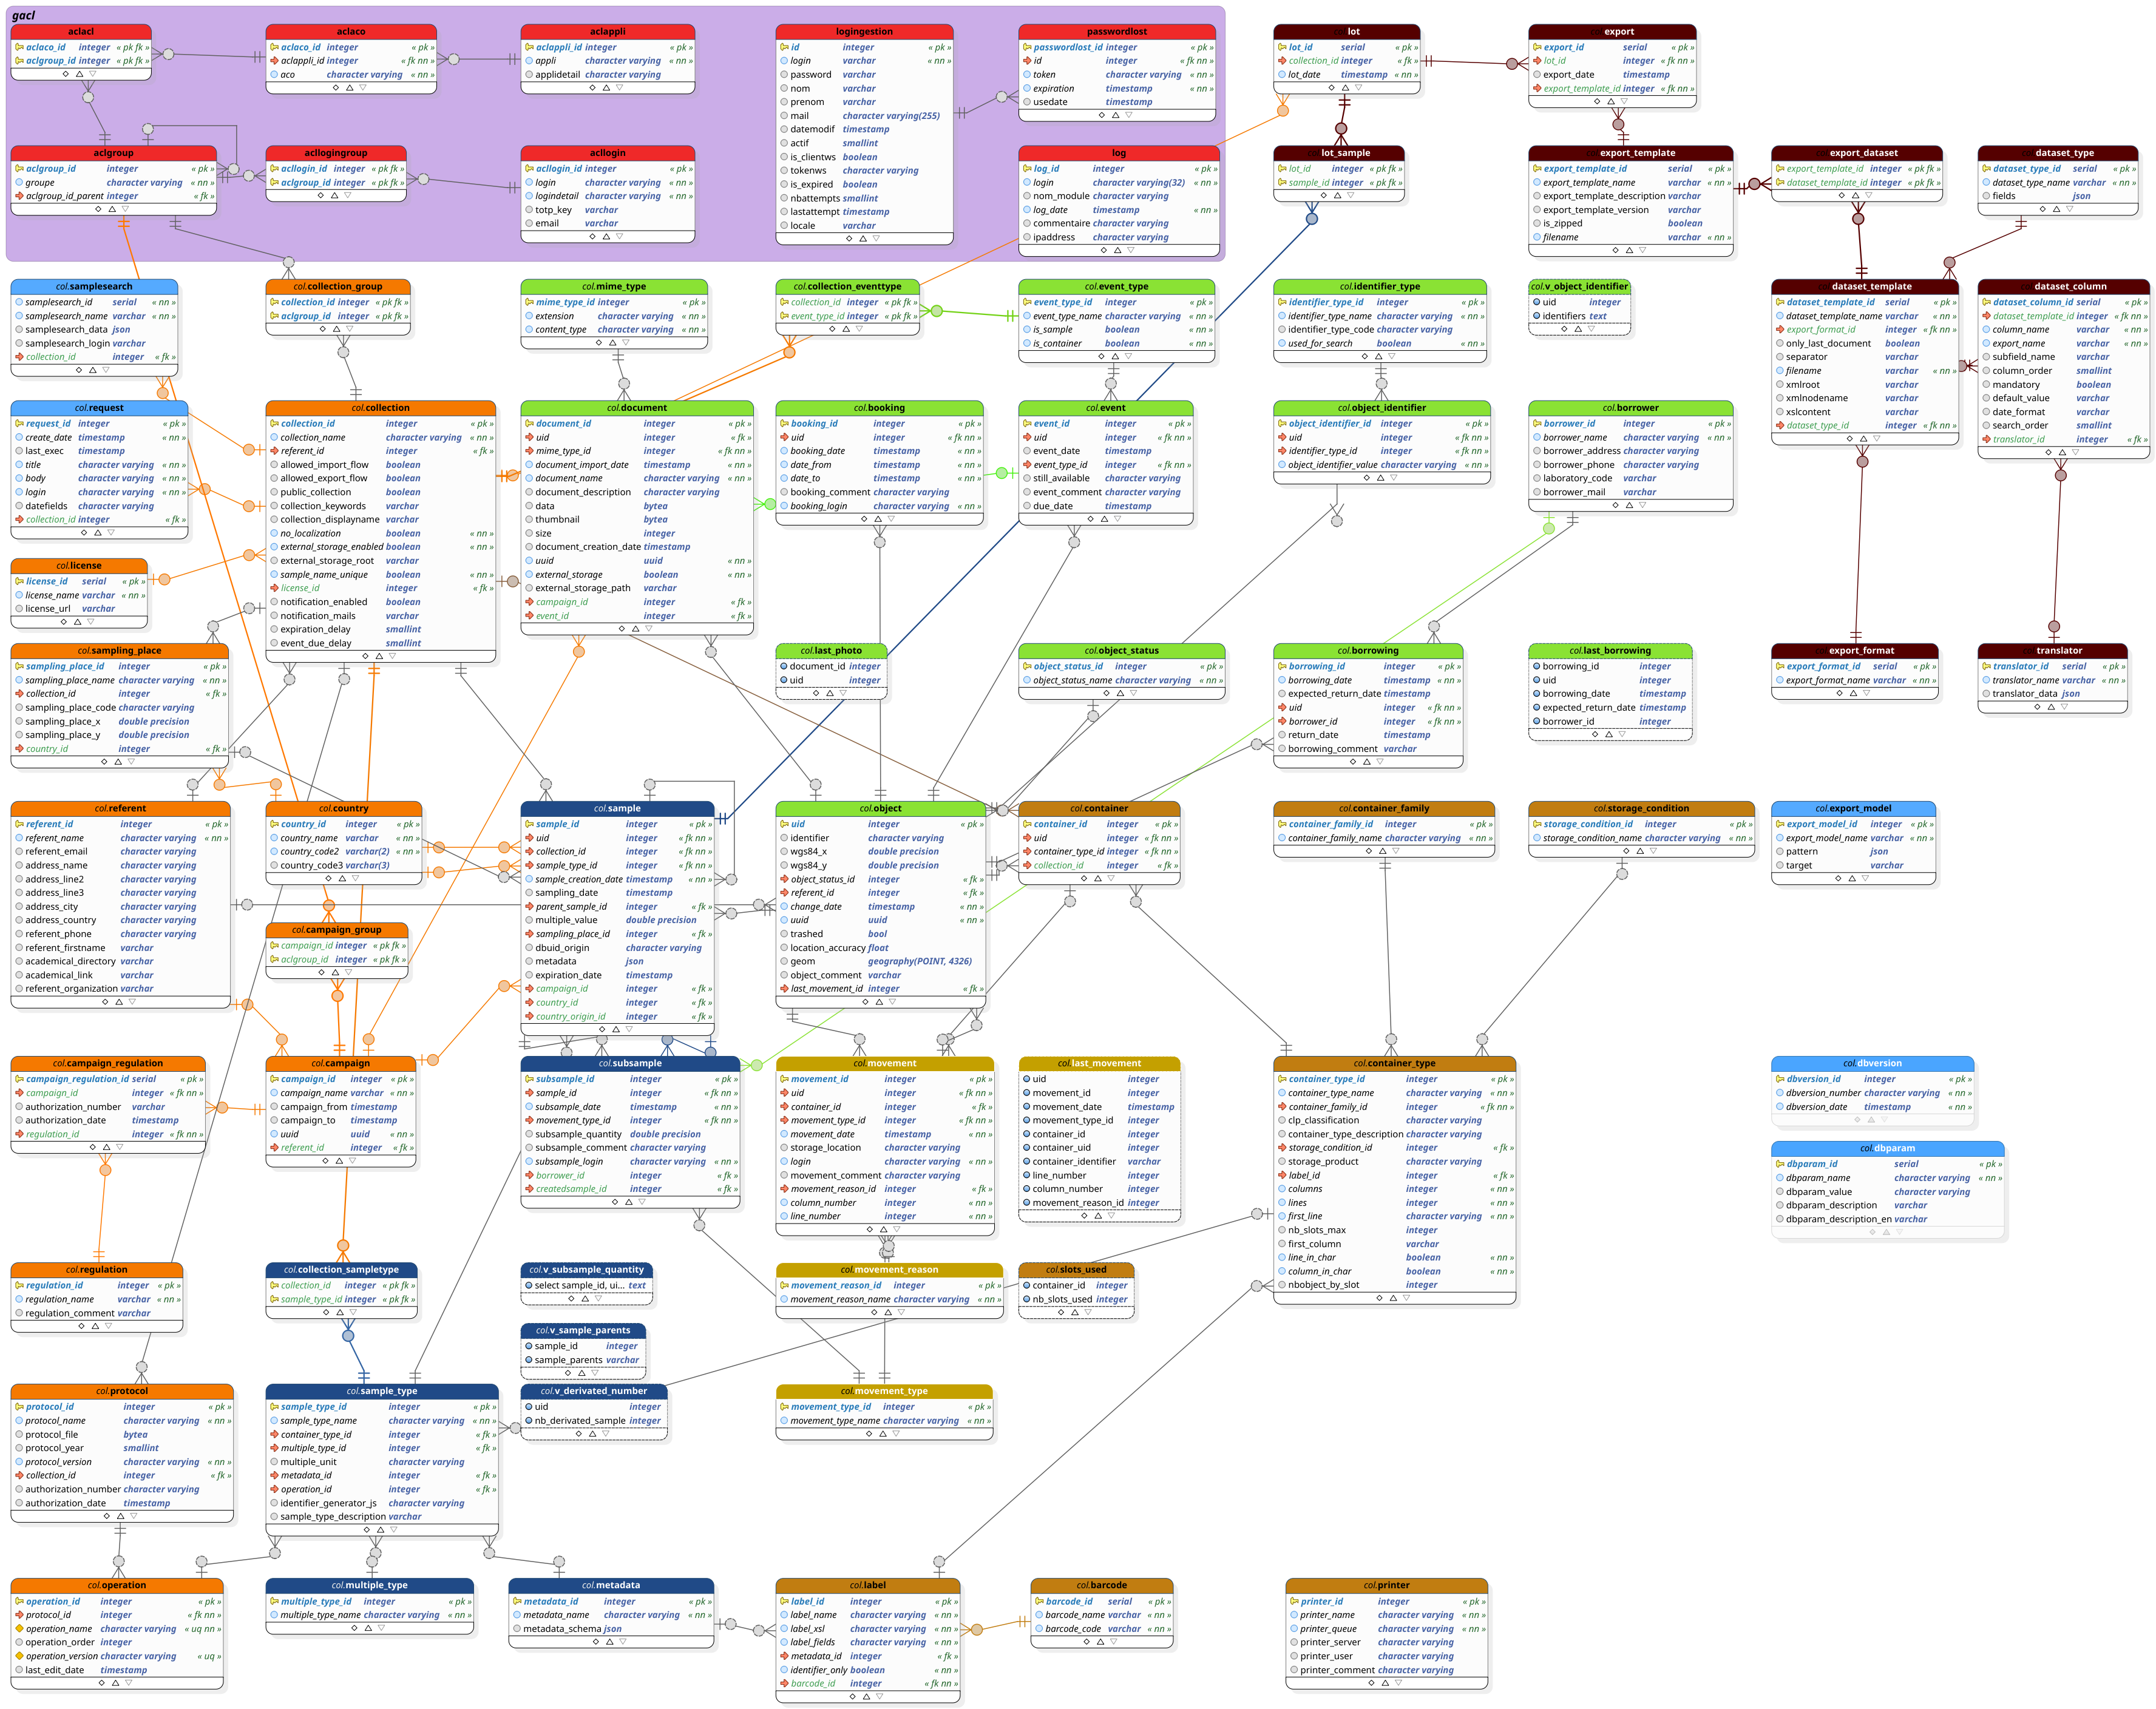
\includegraphics[
width=\textwidth
,angle=90
]{../../collec-schema}


\section{Description des tables}

\subsection{Schema col}
\subsubsection{Tables}
\paragraph{barcode}
Models of barcodes usable

\begin{tabular}{|l| p{2cm}|c|c| p{5cm}|}
\hline
Column name & Type & Not null & Key & Comment \\
\hline
barcode\_id & integer & X & X & \\
barcode\_name & character varying & X &  & Name of the model\\
barcode\_code & character varying & X &  & Value of the barcode used by the generating application, if occures. Default value: QR for QRcode\\
\hline
\end{tabular}
\paragraph{Referenced by}
barcode\_id: col.label (barcode\_id)

\paragraph{booking}
Table of object's bookings

\begin{tabular}{|l| p{2cm}|c|c| p{5cm}|}
\hline
Column name & Type & Not null & Key & Comment \\
\hline
booking\_id & integer & X & X & \\
uid & integer & X &  & \\
booking\_date & timestamp without time zone & X &  & Date of booking\\
date\_from & timestamp without time zone & X &  & Date-time of booking start\\
date\_to & timestamp without time zone & X &  & Date-time of booking end\\
booking\_comment & character varying &  &  & Comment\\
booking\_login & character varying & X &  & Login used to perform the reservation\\
\hline
\end{tabular}
\paragraph{References}
uid: col.object (uid)

\paragraph{borrower}
List of borrowers

\begin{tabular}{|l| p{2cm}|c|c| p{5cm}|}
\hline
Column name & Type & Not null & Key & Comment \\
\hline
borrower\_id & integer & X & X & \\
borrower\_name & character varying & X &  & \\
borrower\_address & character varying &  &  & Address of the borrower\\
borrower\_phone & character varying &  &  & Phone of the contact of the borrower\\
laboratory\_code & character varying &  &  & Laboratory code of the borrower\\
borrower\_mail & character varying &  &  & Mail of the borrower\\
\hline
\end{tabular}
\paragraph{Referenced by}
borrower\_id: col.borrowing (borrower\_id)

\paragraph{borrowing}
List of borrowings

\begin{tabular}{|l| p{2cm}|c|c| p{5cm}|}
\hline
Column name & Type & Not null & Key & Comment \\
\hline
borrowing\_id & integer & X & X & \\
borrowing\_date & timestamp without time zone & X &  & Date of the borrowing\\
expected\_return\_date & timestamp without time zone &  &  & Expected return date of the object\\
uid & integer & X &  & \\
borrower\_id & integer & X &  & \\
return\_date & timestamp without time zone &  &  & Date of return of the object\\
\hline
\end{tabular}
\paragraph{References}
borrower\_id: col.borrower (borrower\_id)

uid: col.object (uid)

\paragraph{campaign}
List of sampling campaigns

\begin{tabular}{|l| p{2cm}|c|c| p{5cm}|}
\hline
Column name & Type & Not null & Key & Comment \\
\hline
campaign\_id & integer & X & X & \\
referent\_id & integer &  &  & \\
campaign\_name & character varying & X &  & Name of the campaign\\
campaign\_from & timestamp without time zone &  &  & Date of start of the campaign\\
campaign\_to & timestamp without time zone &  &  & date of end of the campaign\\
\hline
\end{tabular}
\paragraph{References}
referent\_id: col.referent (referent\_id)

\paragraph{Referenced by}
campaign\_id: col.campaign\_regulation (campaign\_id)

campaign\_id: col.document (campaign\_id)

campaign\_id: col.sample (campaign\_id)

\paragraph{campaign\_regulation}
List of regulations attached to a campaign

\begin{tabular}{|l| p{2cm}|c|c| p{5cm}|}
\hline
Column name & Type & Not null & Key & Comment \\
\hline
campaign\_regulation\_id & integer & X & X & \\
campaign\_id & integer & X &  & \\
regulation\_id & integer & X &  & \\
authorization\_number & character varying &  &  & Number of the authorization\\
authorization\_date & timestamp without time zone &  &  & Date of the authorization\\
\hline
\end{tabular}
\paragraph{References}
campaign\_id: col.campaign (campaign\_id)

regulation\_id: col.regulation (regulation\_id)

\paragraph{collection}
List of all collections into the database

\begin{tabular}{|l| p{2cm}|c|c| p{5cm}|}
\hline
Column name & Type & Not null & Key & Comment \\
\hline
collection\_id & integer & X & X & \\
collection\_name & character varying & X &  & \\
referent\_id & integer &  &  & \\
allowed\_import\_flow & boolean &  &  & Allow an external source to update a collection\\
allowed\_export\_flow & boolean &  &  & Allow interrogation requests from external sources\\
public\_collection & boolean &  &  & Set if a collection can be requested without authentication\\
collection\_keywords & character varying &  &  & List of keywords, separed by a comma\\
collection\_displayname & character varying &  &  & Name used to communicate from the collection, in export module by example\\
license\_id & integer &  &  & \\
\hline
\end{tabular}
\paragraph{References}
license\_id: col.license (license\_id)

referent\_id: col.referent (referent\_id)

\paragraph{Referenced by}
collection\_id: col.lot (collection\_id)

collection\_id: col.samplesearch (collection\_id)

collection\_id: col.sampling\_place (collection\_id)

collection\_id: col.collection\_group (collection\_id)

collection\_id: col.protocol (collection\_id)

collection\_id: col.sample (collection\_id)

\paragraph{collection\_group}
Table of project approvals

\begin{tabular}{|l| p{2cm}|c|c| p{5cm}|}
\hline
Column name & Type & Not null & Key & Comment \\
\hline
collection\_id & integer & X & X & \\
aclgroup\_id & integer & X & X & \\
\hline
\end{tabular}
\paragraph{References}
collection\_id: col.collection (collection\_id)

aclgroup\_id: gacl.aclgroup (aclgroup\_id)

\paragraph{container}
Liste of containers

\begin{tabular}{|l| p{2cm}|c|c| p{5cm}|}
\hline
Column name & Type & Not null & Key & Comment \\
\hline
container\_id & integer & X & X & \\
uid & integer & X &  & \\
container\_type\_id & integer & X &  & \\
\hline
\end{tabular}
\paragraph{References}
container\_type\_id: col.container\_type (container\_type\_id)

uid: col.object (uid)

\paragraph{Referenced by}
container\_id: col.movement (container\_id)

\paragraph{container\_family}
General family of containers

\begin{tabular}{|l| p{2cm}|c|c| p{5cm}|}
\hline
Column name & Type & Not null & Key & Comment \\
\hline
container\_family\_id & integer & X & X & \\
container\_family\_name & character varying & X &  & \\
\hline
\end{tabular}
\paragraph{Referenced by}
container\_family\_id: col.container\_type (container\_family\_id)

\paragraph{container\_type}
Table of types of containers

\begin{tabular}{|l| p{2cm}|c|c| p{5cm}|}
\hline
Column name & Type & Not null & Key & Comment \\
\hline
container\_type\_id & integer & X & X & \\
container\_type\_name & character varying & X &  & \\
container\_family\_id & integer & X &  & \\
clp\_classification & character varying &  &  & Risk classification according to the European CLP directive\\
container\_type\_description & character varying &  &  & Long description\\
storage\_condition\_id & integer &  &  & \\
storage\_product & character varying &  &  & Product used for storage (formol, alcohol...)\\
label\_id & integer &  &  & \\
columns & integer & X &  & Number of storage columns in the container\\
lines & integer & X &  & Number of storage lines in the container\\
first\_line & character varying & X &  & Place of the first line:
T: top
B: bottom\\
nb\_slots\_max & integer &  &  & Number maximum of slots in the container\\
first\_column & character varying &  &  & Place of the first column: 
L: left
R: Right\\
\hline
\end{tabular}
\paragraph{References}
container\_family\_id: col.container\_family (container\_family\_id)

label\_id: col.label (label\_id)

storage\_condition\_id: col.storage\_condition (storage\_condition\_id)

\paragraph{Referenced by}
container\_type\_id: col.container (container\_type\_id)

container\_type\_id: col.sample\_type (container\_type\_id)

\paragraph{country}
List of the countries

\begin{tabular}{|l| p{2cm}|c|c| p{5cm}|}
\hline
Column name & Type & Not null & Key & Comment \\
\hline
country\_id & integer & X & X & Numeric ISO code of the country\\
country\_name & character varying & X &  & Name of the country\\
country\_code2 & character varying(2) & X &  & Code of the country, on 2 positions\\
country\_code3 & character varying(3) &  &  & Code of the country, on 3 positions\\
\hline
\end{tabular}
\paragraph{Referenced by}
country\_id: col.sample (country\_id)

country\_id: col.sampling\_place (country\_id)

country\_id: col.sample (country\_origin\_id)

\paragraph{dataset\_column}
List of columns included into the dataset

\begin{tabular}{|l| p{2cm}|c|c| p{5cm}|}
\hline
Column name & Type & Not null & Key & Comment \\
\hline
dataset\_column\_id & integer & X & X & \\
dataset\_template\_id & integer & X &  & \\
column\_name & character varying & X &  & Name of the column into the database\\
export\_name & character varying & X &  & Name of the column into the export file\\
subfield\_name & character varying &  &  & Name of the field if it into the metadata description of the sample or secondary identifier, etc.\\
translator\_id & integer &  &  & \\
column\_order & smallint &  &  & order of displaying in the exported file\\
mandatory & boolean &  &  & Is the content of the column is mandatory to export data?\\
default\_value & character varying &  &  & Default value, if the value is not filled in\\
date\_format & character varying &  &  & Export date format, in php notation. Example: d/m/Y H:i:s for 25/12/2020 17:15:00\\
search\_order & smallint &  &  & To search a sample, order of the current field to trigger the search\\
\hline
\end{tabular}
\paragraph{References}
dataset\_template\_id: col.dataset\_template (dataset\_template\_id)

translator\_id: col.translator (translator\_id)

\paragraph{dataset\_template}
List of templates of dataset

\begin{tabular}{|l| p{2cm}|c|c| p{5cm}|}
\hline
Column name & Type & Not null & Key & Comment \\
\hline
dataset\_template\_id & integer & X & X & \\
dataset\_template\_name & character varying & X &  & Name of the template\\
export\_format\_id & integer & X &  & \\
dataset\_type\_id & integer & X &  & \\
only\_last\_document & boolean &  &  & If type document, specify if only the last document attached to a sample is exported\\
separator & character varying &  &  & Separator used in csv files (tab , ;)\\
filename & character varying & X &  & File name generated, with extension\\
xmlroot & character varying &  &  & xml root to generate\\
xmlnodename & character varying &  &  & Name of a node in a xml file, for list of samples by example\\
xslcontent & character varying &  &  & Transformation of the generated xml to create a specific xml file\\
\hline
\end{tabular}
\paragraph{References}
dataset\_type\_id: col.dataset\_type (dataset\_type\_id)

export\_format\_id: col.export\_format (export\_format\_id)

\paragraph{Referenced by}
dataset\_template\_id: col.dataset\_column (dataset\_template\_id)

dataset\_template\_id: col.export\_dataset (dataset\_template\_id)

\paragraph{dataset\_type}
Origine of the dataset: sample, collection, document

\begin{tabular}{|l| p{2cm}|c|c| p{5cm}|}
\hline
Column name & Type & Not null & Key & Comment \\
\hline
dataset\_type\_id & integer & X & X & \\
dataset\_type\_name & character varying & X &  & \\
fields & json &  &  & List of allowed fields of the database (json array)\\
\hline
\end{tabular}
\paragraph{Referenced by}
dataset\_type\_id: col.dataset\_template (dataset\_type\_id)

\paragraph{dbparam}
Table of parameters intrinsically associated to the instance

\begin{tabular}{|l| p{2cm}|c|c| p{5cm}|}
\hline
Column name & Type & Not null & Key & Comment \\
\hline
dbparam\_id & integer & X & X & \\
dbparam\_name & character varying & X &  & Name of the parameter\\
dbparam\_value & character varying &  &  & Value of the parameter\\
\hline
\end{tabular}
\paragraph{dbversion}
Table of the database versions

\begin{tabular}{|l| p{2cm}|c|c| p{5cm}|}
\hline
Column name & Type & Not null & Key & Comment \\
\hline
dbversion\_id & integer & X & X & \\
dbversion\_number & character varying & X &  & Number of the version\\
dbversion\_date & timestamp without time zone & X &  & Date of the version\\
\hline
\end{tabular}
\paragraph{document}
Numeric docs associated to an objet or a campaign

\begin{tabular}{|l| p{2cm}|c|c| p{5cm}|}
\hline
Column name & Type & Not null & Key & Comment \\
\hline
document\_id & integer & X & X & \\
uid & integer &  &  & \\
mime\_type\_id & integer & X &  & \\
document\_import\_date & timestamp without time zone & X &  & Import date into the database\\
document\_name & character varying & X &  & Original name\\
document\_description & character varying &  &  & Description\\
data & bytea &  &  & Binary content (object imported)\\
thumbnail & bytea &  &  & Thumbnail in PNG format ( only for pdf, jpg or png docs)\\
size & integer &  &  & Size of downloaded file\\
document\_creation\_date & timestamp without time zone &  &  & Create date of the document (date of photo shooting, for example)\\
campaign\_id & integer &  &  & \\
uuid & uuid & X &  & \\
\hline
\end{tabular}
\paragraph{References}
campaign\_id: col.campaign (campaign\_id)

mime\_type\_id: col.mime\_type (mime\_type\_id)

uid: col.object (uid)

\paragraph{event}
Table of events

\begin{tabular}{|l| p{2cm}|c|c| p{5cm}|}
\hline
Column name & Type & Not null & Key & Comment \\
\hline
event\_id & integer & X & X & \\
uid & integer & X &  & \\
event\_date & timestamp without time zone & X &  & Date-time of the event\\
event\_type\_id & integer & X &  & \\
still\_available & character varying &  &  & still available content in the object, after the event\\
event\_comment & character varying &  &  & Comment\\
\hline
\end{tabular}
\paragraph{References}
event\_type\_id: col.event\_type (event\_type\_id)

uid: col.object (uid)

\paragraph{event\_type}
Event types table

\begin{tabular}{|l| p{2cm}|c|c| p{5cm}|}
\hline
Column name & Type & Not null & Key & Comment \\
\hline
event\_type\_id & integer & X & X & \\
event\_type\_name & character varying & X &  & Name of the type of event\\
is\_sample & boolean & X &  & The event is applicable to the samples\\
is\_container & boolean & X &  & The event is applicable to the containers\\
\hline
\end{tabular}
\paragraph{Referenced by}
event\_type\_id: col.event (event\_type\_id)

\paragraph{export}
List of exports processed

\begin{tabular}{|l| p{2cm}|c|c| p{5cm}|}
\hline
Column name & Type & Not null & Key & Comment \\
\hline
export\_id & integer & X & X & \\
lot\_id & integer & X &  & \\
export\_date & timestamp without time zone &  &  & Date of last execution of the export\\
export\_template\_id & integer & X &  & \\
\hline
\end{tabular}
\paragraph{References}
export\_template\_id: col.export\_template (export\_template\_id)

lot\_id: col.lot (lot\_id)

\paragraph{export\_dataset}
List of datasets embedded into the template of export

\begin{tabular}{|l| p{2cm}|c|c| p{5cm}|}
\hline
Column name & Type & Not null & Key & Comment \\
\hline
export\_template\_id & integer & X & X & \\
dataset\_template\_id & integer & X & X & \\
\hline
\end{tabular}
\paragraph{References}
dataset\_template\_id: col.dataset\_template (dataset\_template\_id)

export\_template\_id: col.export\_template (export\_template\_id)

\paragraph{export\_format}
List of formats of export

\begin{tabular}{|l| p{2cm}|c|c| p{5cm}|}
\hline
Column name & Type & Not null & Key & Comment \\
\hline
export\_format\_id & integer & X & X & \\
export\_format\_name & character varying & X &  & \\
\hline
\end{tabular}
\paragraph{Referenced by}
export\_format\_id: col.dataset\_template (export\_format\_id)

\paragraph{export\_model}
Structure of an export/import of table data

\begin{tabular}{|l| p{2cm}|c|c| p{5cm}|}
\hline
Column name & Type & Not null & Key & Comment \\
\hline
export\_model\_id & integer & X & X & \\
export\_model\_name & character varying & X &  & Name of the structure of export\\
pattern & json &  &  & Pattern of the export/import.
Structure:
[{technicalKey:string,businessKey:string,tableName:string,tableAlias:string,children[table1,table2],parentKey:string,secondaryParentKey:string}]\\
target & character varying &  &  & Main table targetted\\
\hline
\end{tabular}
\paragraph{export\_template}
List of models of export

\begin{tabular}{|l| p{2cm}|c|c| p{5cm}|}
\hline
Column name & Type & Not null & Key & Comment \\
\hline
export\_template\_id & integer & X & X & \\
export\_template\_name & character varying & X &  & Name of the model\\
export\_template\_description & character varying &  &  & Description of the model\\
export\_template\_version & character varying &  &  & Version of the model, if necessary\\
is\_zipped & boolean &  &  & Specify if the generated files must be zipped\\
filename & character varying & X &  & Name of the file generated\\
\hline
\end{tabular}
\paragraph{Referenced by}
export\_template\_id: col.export (export\_template\_id)

export\_template\_id: col.export\_dataset (export\_template\_id)

\paragraph{identifier\_type}
Table of identifier types

\begin{tabular}{|l| p{2cm}|c|c| p{5cm}|}
\hline
Column name & Type & Not null & Key & Comment \\
\hline
identifier\_type\_id & integer & X & X & \\
identifier\_type\_name & character varying & X &  & Textual name of the identifier\\
identifier\_type\_code & character varying &  &  & Identifier code, used in the labels\\
used\_for\_search & boolean & X &  & Is the identifier usable for barcode searches?\\
\hline
\end{tabular}
\paragraph{Referenced by}
identifier\_type\_id: col.object\_identifier (identifier\_type\_id)

\paragraph{label}
Table of label models

\begin{tabular}{|l| p{2cm}|c|c| p{5cm}|}
\hline
Column name & Type & Not null & Key & Comment \\
\hline
label\_id & integer & X & X & \\
label\_name & character varying & X &  & Name of the model\\
label\_xsl & character varying & X &  & XSL content used by FOP transformation (https://xmlgraphics.apache.org/fop/)\\
label\_fields & character varying & X &  & List of fields incorporated in the QRCODE\\
metadata\_id & integer &  &  & Model of the metadata template associated with this label\\
identifier\_only & boolean & X &  & true: the qrcode contains only a business identifier\\
barcode\_id & integer & X &  & \\
\hline
\end{tabular}
\paragraph{References}
barcode\_id: col.barcode (barcode\_id)

metadata\_id: col.metadata (metadata\_id)

\paragraph{Referenced by}
label\_id: col.container\_type (label\_id)

\paragraph{license}
List of licenses usable to communicate informations on the collections

\begin{tabular}{|l| p{2cm}|c|c| p{5cm}|}
\hline
Column name & Type & Not null & Key & Comment \\
\hline
license\_id & integer & X & X & \\
license\_name & character varying & X &  & Name of the license\\
license\_url & character varying &  &  & Link of download of the text of the license\\
\hline
\end{tabular}
\paragraph{Referenced by}
license\_id: col.collection (license\_id)

\paragraph{lot}
List of lots of export

\begin{tabular}{|l| p{2cm}|c|c| p{5cm}|}
\hline
Column name & Type & Not null & Key & Comment \\
\hline
lot\_id & integer & X & X & \\
collection\_id & integer &  &  & \\
lot\_date & timestamp without time zone & X &  & Date of creation of the lot\\
\hline
\end{tabular}
\paragraph{References}
collection\_id: col.collection (collection\_id)

\paragraph{Referenced by}
lot\_id: col.export (lot\_id)

lot\_id: col.lot\_sample (lot\_id)

\paragraph{lot\_sample}
List of samples associated into a lot

\begin{tabular}{|l| p{2cm}|c|c| p{5cm}|}
\hline
Column name & Type & Not null & Key & Comment \\
\hline
lot\_id & integer & X & X & \\
sample\_id & integer & X & X & \\
\hline
\end{tabular}
\paragraph{References}
lot\_id: col.lot (lot\_id)

sample\_id: col.sample (sample\_id)

\paragraph{metadata}
Table of metadata usable with types of samples

\begin{tabular}{|l| p{2cm}|c|c| p{5cm}|}
\hline
Column name & Type & Not null & Key & Comment \\
\hline
metadata\_id & integer & X & X & \\
metadata\_name & character varying & X &  & Name of the metadata set\\
metadata\_schema & json &  &  & JSON schema of the metadata form\\
\hline
\end{tabular}
\paragraph{Referenced by}
metadata\_id: col.label (metadata\_id)

metadata\_id: col.sample\_type (metadata\_id)

\paragraph{mime\_type}
Mime types of imported files

\begin{tabular}{|l| p{2cm}|c|c| p{5cm}|}
\hline
Column name & Type & Not null & Key & Comment \\
\hline
mime\_type\_id & integer & X & X & \\
extension & character varying & X &  & File extension\\
content\_type & character varying & X &  & Official mime type\\
\hline
\end{tabular}
\paragraph{Referenced by}
mime\_type\_id: col.document (mime\_type\_id)

\paragraph{movement}
Records of objects movements

\begin{tabular}{|l| p{2cm}|c|c| p{5cm}|}
\hline
Column name & Type & Not null & Key & Comment \\
\hline
movement\_id & integer & X & X & \\
uid & integer & X &  & \\
container\_id & integer &  &  & \\
movement\_type\_id & integer & X &  & \\
movement\_date & timestamp without time zone & X &  & Date-time of the movement\\
storage\_location & character varying &  &  & Place of the object in the container, in textual form\\
login & character varying & X &  & Name of the operator who performed the operation\\
movement\_comment & character varying &  &  & Comment\\
movement\_reason\_id & integer &  &  & \\
column\_number & integer & X &  & Number of the storage column in the container\\
line\_number & integer & X &  & Number of the storage line in the container\\
\hline
\end{tabular}
\paragraph{References}
container\_id: col.container (container\_id)

movement\_reason\_id: col.movement\_reason (movement\_reason\_id)

movement\_type\_id: col.movement\_type (movement\_type\_id)

uid: col.object (uid)

\paragraph{movement\_reason}
List of the reasons of the movement

\begin{tabular}{|l| p{2cm}|c|c| p{5cm}|}
\hline
Column name & Type & Not null & Key & Comment \\
\hline
movement\_reason\_id & integer & X & X & \\
movement\_reason\_name & character varying & X &  & \\
\hline
\end{tabular}
\paragraph{Referenced by}
movement\_reason\_id: col.movement (movement\_reason\_id)

\paragraph{movement\_type}
Type de mouvement

\begin{tabular}{|l| p{2cm}|c|c| p{5cm}|}
\hline
Column name & Type & Not null & Key & Comment \\
\hline
movement\_type\_id & integer & X & X & \\
movement\_type\_name & character varying & X &  & \\
\hline
\end{tabular}
\paragraph{Referenced by}
movement\_type\_id: col.movement (movement\_type\_id)

movement\_type\_id: col.subsample (movement\_type\_id)

\paragraph{multiple\_type}
Table of categories of potential sub-sampling (unit, quantity, percentage, etc.)

\begin{tabular}{|l| p{2cm}|c|c| p{5cm}|}
\hline
Column name & Type & Not null & Key & Comment \\
\hline
multiple\_type\_id & integer & X & X & \\
multiple\_type\_name & character varying & X &  & \\
\hline
\end{tabular}
\paragraph{Referenced by}
multiple\_type\_id: col.sample\_type (multiple\_type\_id)

\paragraph{object}
Table of objects

\begin{tabular}{|l| p{2cm}|c|c| p{5cm}|}
\hline
Column name & Type & Not null & Key & Comment \\
\hline
uid & integer & X & X & Unique identifier in the database of all objects\\
identifier & character varying &  &  & Main working identifier\\
wgs84\_x & double precision &  &  & GPS longitude, in decimal form\\
wgs84\_y & double precision &  &  & GPS latitude, in decimal form\\
object\_status\_id & integer &  &  & \\
referent\_id & integer &  &  & \\
change\_date & timestamp without time zone & X &  & Technical date of changement of the object\\
uuid & uuid & X &  & UUID of the object\\
trashed & boolean &  &  & If the object is trashed before completly destroyed ?\\
location\_accuracy & double precision &  &  & Location accuracy of the object, in meters\\
geom & geography(Point,4326) &  &  & Geographic point generate from wgs84\_x and wgs84\_y\\
object\_comment & character varying &  &  & Comment on the object (sample or container)\\
\hline
\end{tabular}
\paragraph{References}
object\_status\_id: col.object\_status (object\_status\_id)

referent\_id: col.referent (referent\_id)

\paragraph{Referenced by}
uid: col.booking (uid)

uid: col.container (uid)

uid: col.document (uid)

uid: col.event (uid)

uid: col.borrowing (uid)

uid: col.object\_identifier (uid)

uid: col.sample (uid)

uid: col.movement (uid)

\paragraph{object\_identifier}
Table of complementary identifiers

\begin{tabular}{|l| p{2cm}|c|c| p{5cm}|}
\hline
Column name & Type & Not null & Key & Comment \\
\hline
object\_identifier\_id & integer & X & X & \\
uid & integer & X &  & \\
identifier\_type\_id & integer & X &  & \\
object\_identifier\_value & character varying & X &  & Identifier value\\
\hline
\end{tabular}
\paragraph{References}
identifier\_type\_id: col.identifier\_type (identifier\_type\_id)

uid: col.object (uid)

\paragraph{object\_status}
Table of types of status

\begin{tabular}{|l| p{2cm}|c|c| p{5cm}|}
\hline
Column name & Type & Not null & Key & Comment \\
\hline
object\_status\_id & integer & X & X & \\
object\_status\_name & character varying & X &  & \\
\hline
\end{tabular}
\paragraph{Referenced by}
object\_status\_id: col.object (object\_status\_id)

\paragraph{operation}
List of operations attached to a protocol

\begin{tabular}{|l| p{2cm}|c|c| p{5cm}|}
\hline
Column name & Type & Not null & Key & Comment \\
\hline
operation\_id & integer & X & X & \\
protocol\_id & integer & X &  & \\
operation\_name & character varying & X &  & \\
operation\_order & integer &  &  & Order to perform the operation in the protocol\\
operation\_version & character varying &  &  & Version of the operation\\
last\_edit\_date & timestamp without time zone &  &  & Last edit date of the operation\\
\hline
\end{tabular}
\paragraph{References}
protocol\_id: col.protocol (protocol\_id)

\paragraph{Referenced by}
operation\_id: col.sample\_type (operation\_id)

\paragraph{printer}
Table of printers directly managed by the server

\begin{tabular}{|l| p{2cm}|c|c| p{5cm}|}
\hline
Column name & Type & Not null & Key & Comment \\
\hline
printer\_id & integer & X & X & \\
printer\_name & character varying & X &  & Usual name of the printer, displayed in the forms\\
printer\_queue & character varying & X &  & Name of the printer known by the operating system of the server\\
printer\_server & character varying &  &  & Server address, if the printer is not connected at the localhost\\
printer\_user & character varying &  &  & User used to print, if necessary\\
printer\_comment & character varying &  &  & Comment\\
\hline
\end{tabular}
\paragraph{protocol}
List of protocols

\begin{tabular}{|l| p{2cm}|c|c| p{5cm}|}
\hline
Column name & Type & Not null & Key & Comment \\
\hline
protocol\_id & integer & X & X & \\
protocol\_name & character varying & X &  & Name of the protocol\\
protocol\_file & bytea &  &  & PDF description of the protocol\\
protocol\_year & smallint &  &  & Year of the protocol\\
protocol\_version & character varying & X &  & Version of the protocol\\
collection\_id & integer &  &  & \\
authorization\_number & character varying &  &  & Number of the prelevement authorization\\
authorization\_date & timestamp without time zone &  &  & Date of the prelevement authorization\\
\hline
\end{tabular}
\paragraph{References}
collection\_id: col.collection (collection\_id)

\paragraph{Referenced by}
protocol\_id: col.operation (protocol\_id)

\paragraph{referent}
Table of sample referents

\begin{tabular}{|l| p{2cm}|c|c| p{5cm}|}
\hline
Column name & Type & Not null & Key & Comment \\
\hline
referent\_id & integer & X & X & \\
referent\_name & character varying & X &  & Name, firstname-lastname or department name\\
referent\_email & character varying &  &  & Email for contact\\
address\_name & character varying &  &  & Name for postal address\\
address\_line2 & character varying &  &  & second line in postal address\\
address\_line3 & character varying &  &  & third line in postal address\\
address\_city & character varying &  &  & ZIPCode and City in postal address\\
address\_country & character varying &  &  & Country in postal address\\
referent\_phone & character varying &  &  & Contact phone\\
referent\_firstname & character varying &  &  & Firstname of the referent\\
academical\_directory & character varying &  &  & Academical directory used to identifier the referent, as https://orcid.org or https://www.researchgate.net\\
academical\_link & character varying &  &  & Link used to identify the referent, as https://orcid.org/0000-0003-4207-4107\\
\hline
\end{tabular}
\paragraph{Referenced by}
referent\_id: col.collection (referent\_id)

referent\_id: col.campaign (referent\_id)

referent\_id: col.object (referent\_id)

\paragraph{regulation}
Table of regulations

\begin{tabular}{|l| p{2cm}|c|c| p{5cm}|}
\hline
Column name & Type & Not null & Key & Comment \\
\hline
regulation\_id & integer & X & X & \\
regulation\_name & character varying & X &  & Name of the regulation\\
regulation\_comment & character varying &  &  & regulatory clarity\\
\hline
\end{tabular}
\paragraph{Referenced by}
regulation\_id: col.campaign\_regulation (regulation\_id)

\paragraph{request}
Request table in database

\begin{tabular}{|l| p{2cm}|c|c| p{5cm}|}
\hline
Column name & Type & Not null & Key & Comment \\
\hline
request\_id & integer & X & X & \\
create\_date & timestamp without time zone & X &  & Date of create of the request\\
last\_exec & timestamp without time zone &  &  & Date of the last execution\\
title & character varying & X &  & Title of the request\\
body & character varying & X &  & Body of the request. Don't begin it by SELECT, which will be added automatically\\
login & character varying & X &  & Login of the creator of the request\\
datefields & character varying &  &  & List of the date fields used in the request, separated by a comma, for format it\\
\hline
\end{tabular}
\paragraph{sample}
Table of samples

\begin{tabular}{|l| p{2cm}|c|c| p{5cm}|}
\hline
Column name & Type & Not null & Key & Comment \\
\hline
sample\_id & integer & X & X & \\
uid & integer & X &  & \\
collection\_id & integer & X &  & \\
sample\_type\_id & integer & X &  & \\
sample\_creation\_date & timestamp without time zone & X &  & Creation date of the record in the database\\
sampling\_date & timestamp without time zone &  &  & Creation date of the physical sample or date of sampling\\
parent\_sample\_id & integer &  &  & \\
multiple\_value & double precision &  &  & \\
sampling\_place\_id & integer &  &  & \\
dbuid\_origin & character varying &  &  & Reference used in the original database, under the form db:uid. Used for read the labels created in others instances\\
metadata & json &  &  & Metadata associated with the sample, in JSON format\\
expiration\_date & timestamp without time zone &  &  & Date of expiration of the sample. After this date, the sample is not usable\\
campaign\_id & integer &  &  & \\
country\_id & integer &  &  & \\
country\_origin\_id & integer &  &  & \\
\hline
\end{tabular}
\paragraph{References}
campaign\_id: col.campaign (campaign\_id)

collection\_id: col.collection (collection\_id)

country\_id: col.country (country\_id)

country\_origin\_id: col.country (country\_id)

uid: col.object (uid)

parent\_sample\_id: col.sample (sample\_id)

sample\_type\_id: col.sample\_type (sample\_type\_id)

sampling\_place\_id: col.sampling\_place (sampling\_place\_id)

\paragraph{Referenced by}
sample\_id: col.lot\_sample (sample\_id)

sample\_id: col.sample (parent\_sample\_id)

sample\_id: col.subsample (sample\_id)

\paragraph{sample\_type}
Table of the types of samples

\begin{tabular}{|l| p{2cm}|c|c| p{5cm}|}
\hline
Column name & Type & Not null & Key & Comment \\
\hline
sample\_type\_id & integer & X & X & \\
sample\_type\_name & character varying & X &  & Name of the type\\
container\_type\_id & integer &  &  & \\
multiple\_type\_id & integer &  &  & \\
multiple\_unit & character varying &  &  & Name of the unit used  to qualify the number of sub-samples (ml, number, g, etc.)\\
metadata\_id & integer &  &  & \\
operation\_id & integer &  &  & \\
identifier\_generator\_js & character varying &  &  & Javascript function code used to automaticaly generate a working identifier from the intered information\\
sample\_type\_description & character varying &  &  & Description of the type of sample\\
\hline
\end{tabular}
\paragraph{References}
container\_type\_id: col.container\_type (container\_type\_id)

metadata\_id: col.metadata (metadata\_id)

multiple\_type\_id: col.multiple\_type (multiple\_type\_id)

operation\_id: col.operation (operation\_id)

\paragraph{Referenced by}
sample\_type\_id: col.sample (sample\_type\_id)

\paragraph{samplesearch}
List of sample saved search

\begin{tabular}{|l| p{2cm}|c|c| p{5cm}|}
\hline
Column name & Type & Not null & Key & Comment \\
\hline
samplesearch\_id & integer & X &  & \\
samplesearch\_name & character varying & X &  & Name of the search parameters\\
samplesearch\_data & json &  &  & List of all research parameters\\
samplesearch\_login & character varying &  &  & Login of the creator\\
collection\_id & integer &  &  & \\
\hline
\end{tabular}
\paragraph{References}
collection\_id: col.collection (collection\_id)

\paragraph{sampling\_place}
Table of sampling places

\begin{tabular}{|l| p{2cm}|c|c| p{5cm}|}
\hline
Column name & Type & Not null & Key & Comment \\
\hline
sampling\_place\_id & integer & X & X & \\
sampling\_place\_name & character varying & X &  & Name of the sampling place\\
collection\_id & integer &  &  & Collection of rattachment\\
sampling\_place\_code & character varying &  &  & Working code of the station\\
sampling\_place\_x & double precision &  &  & Longitude of the station, in WGS84\\
sampling\_place\_y & double precision &  &  & Latitude of the station, in WGS84\\
country\_id & integer &  &  & \\
\hline
\end{tabular}
\paragraph{References}
collection\_id: col.collection (collection\_id)

country\_id: col.country (country\_id)

\paragraph{Referenced by}
sampling\_place\_id: col.sample (sampling\_place\_id)

\paragraph{storage\_condition}
Table of the conditions of storage

\begin{tabular}{|l| p{2cm}|c|c| p{5cm}|}
\hline
Column name & Type & Not null & Key & Comment \\
\hline
storage\_condition\_id & integer & X & X & \\
storage\_condition\_name & character varying & X &  & \\
\hline
\end{tabular}
\paragraph{Referenced by}
storage\_condition\_id: col.container\_type (storage\_condition\_id)

\paragraph{subsample}
Table of sub-sample takes and returns

\begin{tabular}{|l| p{2cm}|c|c| p{5cm}|}
\hline
Column name & Type & Not null & Key & Comment \\
\hline
subsample\_id & integer & X & X & \\
sample\_id & integer & X &  & \\
subsample\_date & timestamp without time zone & X &  & Date-time of the operation\\
movement\_type\_id & integer & X &  & \\
subsample\_quantity & double precision &  &  & Quantity taken or returned\\
subsample\_comment & character varying &  &  & Comment on this operation\\
subsample\_login & character varying & X &  & Login of the user who perform this operation\\
\hline
\end{tabular}
\paragraph{References}
movement\_type\_id: col.movement\_type (movement\_type\_id)

sample\_id: col.sample (sample\_id)

\paragraph{translator}
Table of translator of values

\begin{tabular}{|l| p{2cm}|c|c| p{5cm}|}
\hline
Column name & Type & Not null & Key & Comment \\
\hline
translator\_id & integer & X & X & \\
translator\_name & character varying & X &  & \\
translator\_data & json &  &  & List of translations under the form term\_in\_database:term\_in\_the\_export\_file\\
\hline
\end{tabular}
\paragraph{Referenced by}
translator\_id: col.dataset\_column (translator\_id)

\subsubsection{Views}
\paragraph{last\_borrowing}
 SELECT b1.borrowing\_id,
    b1.uid,
    b1.borrowing\_date,
    b1.expected\_return\_date,
    b1.borrower\_id
   FROM col.borrowing b1
  WHERE (b1.borrowing\_id = ( SELECT b2.borrowing\_id
           FROM col.borrowing b2
          WHERE ((b1.uid = b2.uid) AND (b2.return\_date IS NULL))
          ORDER BY b2.borrowing\_date DESC
         LIMIT 1));

\begin{tabular}{|l| p{2cm}|c|c| p{5cm}|}
\hline
Column name & Type \\
\hline
borrowing\_id & integer\\
uid & integer\\
borrowing\_date & timestamp without time zone\\
expected\_return\_date & timestamp without time zone\\
borrower\_id & integer\\
\hline
\end{tabular}
\paragraph{last\_movement}
 SELECT s.uid,
    s.movement\_id,
    s.movement\_date,
    s.movement\_type\_id,
    s.container\_id,
    c.uid AS container\_uid,
    s.line\_number,
    s.column\_number,
    s.movement\_reason\_id
   FROM (col.movement s
     LEFT JOIN col.container c USING (container\_id))
  WHERE (s.movement\_id = ( SELECT st.movement\_id
           FROM col.movement st
          WHERE (s.uid = st.uid)
          ORDER BY st.movement\_date DESC
         LIMIT 1));

\begin{tabular}{|l| p{2cm}|c|c| p{5cm}|}
\hline
Column name & Type \\
\hline
uid & integer\\
movement\_id & integer\\
movement\_date & timestamp without time zone\\
movement\_type\_id & integer\\
container\_id & integer\\
container\_uid & integer\\
line\_number & integer\\
column\_number & integer\\
movement\_reason\_id & integer\\
\hline
\end{tabular}
\paragraph{last\_photo}
 SELECT d.document\_id,
    d.uid
   FROM col.document d
  WHERE (d.document\_id = ( SELECT d1.document\_id
           FROM col.document d1
          WHERE ((d1.mime\_type\_id = ANY (ARRAY[4, 5, 6])) AND (d.uid = d1.uid))
          ORDER BY d1.document\_creation\_date DESC, d1.document\_import\_date DESC, d1.document\_id DESC
         LIMIT 1));

\begin{tabular}{|l| p{2cm}|c|c| p{5cm}|}
\hline
Column name & Type \\
\hline
document\_id & integer\\
uid & integer\\
\hline
\end{tabular}
\paragraph{slots\_used}
 SELECT last\_movement.container\_id,
    count(*) AS nb\_slots\_used
   FROM col.last\_movement
  WHERE (last\_movement.movement\_type\_id = 1)
  GROUP BY last\_movement.container\_id;

\begin{tabular}{|l| p{2cm}|c|c| p{5cm}|}
\hline
Column name & Type \\
\hline
container\_id & integer\\
nb\_slots\_used & bigint\\
\hline
\end{tabular}
\paragraph{v\_object\_identifier}
 SELECT object\_identifier.uid,
    array\_to\_string(array\_agg((((
        CASE
            WHEN (identifier\_type.identifier\_type\_code IS NOT NULL) THEN identifier\_type.identifier\_type\_code
            ELSE identifier\_type.identifier\_type\_name
        END)::text || ':'::text) || (object\_identifier.object\_identifier\_value)::text) ORDER BY identifier\_type.identifier\_type\_code, object\_identifier.object\_identifier\_value), ','::text) AS identifiers
   FROM (col.object\_identifier
     JOIN col.identifier\_type USING (identifier\_type\_id))
  GROUP BY object\_identifier.uid
  ORDER BY object\_identifier.uid;

\begin{tabular}{|l| p{2cm}|c|c| p{5cm}|}
\hline
Column name & Type \\
\hline
uid & integer\\
identifiers & text\\
\hline
\end{tabular}
\paragraph{v\_subsample\_quantity}
 SELECT s.sample\_id,
    s.uid,
    s.multiple\_value,
    COALESCE(( SELECT sum(smore.subsample\_quantity) AS sum
           FROM col.subsample smore
          WHERE ((smore.movement\_type\_id = 1) AND (smore.sample\_id = s.sample\_id))), (0)::double precision) AS subsample\_more,
    COALESCE(( SELECT sum(sless.subsample\_quantity) AS sum
           FROM col.subsample sless
          WHERE ((sless.movement\_type\_id = 2) AND (sless.sample\_id = s.sample\_id))), (0)::double precision) AS subsample\_less
   FROM col.sample s;

\begin{tabular}{|l| p{2cm}|c|c| p{5cm}|}
\hline
Column name & Type \\
\hline
sample\_id & integer\\
uid & integer\\
multiple\_value & double precision\\
subsample\_more & double precision\\
subsample\_less & double precision\\
\hline
\end{tabular}
\subsection{Schema gacl}
\subsubsection{Tables}
\paragraph{aclacl}
Table of rights granted

\begin{tabular}{|l| p{2cm}|c|c| p{5cm}|}
\hline
Column name & Type & Not null & Key & Comment \\
\hline
aclaco\_id & integer & X & X & \\
aclgroup\_id & integer & X & X & \\
\hline
\end{tabular}
\paragraph{References}
aclaco\_id: gacl.aclaco (aclaco\_id)

aclgroup\_id: gacl.aclgroup (aclgroup\_id)

\paragraph{aclaco}
Table of managed rights

\begin{tabular}{|l| p{2cm}|c|c| p{5cm}|}
\hline
Column name & Type & Not null & Key & Comment \\
\hline
aclaco\_id & integer & X & X & \\
aclappli\_id & integer & X &  & \\
aco & character varying & X &  & Name of the right in the application\\
\hline
\end{tabular}
\paragraph{References}
aclappli\_id: gacl.aclappli (aclappli\_id)

\paragraph{Referenced by}
aclaco\_id: gacl.aclacl (aclaco\_id)

\paragraph{aclappli}
Table of managed applications

\begin{tabular}{|l| p{2cm}|c|c| p{5cm}|}
\hline
Column name & Type & Not null & Key & Comment \\
\hline
aclappli\_id & integer & X & X & \\
appli & character varying & X &  & Code of the application used to manage the rights\\
applidetail & character varying &  &  & Description of the application\\
\hline
\end{tabular}
\paragraph{Referenced by}
aclappli\_id: gacl.aclaco (aclappli\_id)

\paragraph{aclgroup}
Groups of logins

\begin{tabular}{|l| p{2cm}|c|c| p{5cm}|}
\hline
Column name & Type & Not null & Key & Comment \\
\hline
aclgroup\_id & integer & X & X & \\
groupe & character varying & X &  & Name of the group\\
aclgroup\_id\_parent & integer &  &  & Parent group who inherits of the rights attributed to this group\\
\hline
\end{tabular}
\paragraph{References}
aclgroup\_id\_parent: gacl.aclgroup (aclgroup\_id)

\paragraph{Referenced by}
aclgroup\_id: gacl.aclacl (aclgroup\_id)

aclgroup\_id: gacl.aclgroup (aclgroup\_id\_parent)

aclgroup\_id: gacl.acllogingroup (aclgroup\_id)

aclgroup\_id: col.collection\_group (aclgroup\_id)

\paragraph{acllogin}
List of logins granted to access to the modules of the application

\begin{tabular}{|l| p{2cm}|c|c| p{5cm}|}
\hline
Column name & Type & Not null & Key & Comment \\
\hline
acllogin\_id & integer & X & X & \\
login & character varying & X &  & Login. It must be the same as the table logingestion\\
logindetail & character varying & X &  & Displayed name\\
totp\_key & character varying &  &  & TOTP secret key for the user\\
\hline
\end{tabular}
\paragraph{Referenced by}
acllogin\_id: gacl.acllogingroup (acllogin\_id)

\paragraph{acllogingroup}
List of logins in the groups

\begin{tabular}{|l| p{2cm}|c|c| p{5cm}|}
\hline
Column name & Type & Not null & Key & Comment \\
\hline
acllogin\_id & integer & X & X & \\
aclgroup\_id & integer & X & X & \\
\hline
\end{tabular}
\paragraph{References}
aclgroup\_id: gacl.aclgroup (aclgroup\_id)

acllogin\_id: gacl.acllogin (acllogin\_id)

\paragraph{log}
List of all recorded operations (logins, calls of modules, etc.)

\begin{tabular}{|l| p{2cm}|c|c| p{5cm}|}
\hline
Column name & Type & Not null & Key & Comment \\
\hline
log\_id & integer & X & X & \\
login & character varying(32) & X &  & Code of the login who performs the operation\\
nom\_module & character varying &  &  & Name of the performed module\\
log\_date & timestamp without time zone & X &  & Date-time of the operation\\
commentaire & character varying &  &  & Complementary data recorded\\
ipaddress & character varying &  &  & IP address of the client\\
\hline
\end{tabular}
\paragraph{logingestion}
List of logins used to connect to the application, when the account is managed by the application itself. This table also contains the accounts authorized to use the web services.

\begin{tabular}{|l| p{2cm}|c|c| p{5cm}|}
\hline
Column name & Type & Not null & Key & Comment \\
\hline
id & integer & X & X & \\
login & character varying & X &  & Login used by the user\\
password & character varying &  &  & \\
nom & character varying &  &  & Name of the user\\
prenom & character varying &  &  & Surname\\
mail & character varying(255) &  &  & email. Used to send password loss messages\\
datemodif & timestamp without time zone &  &  & Last date of change of the record\\
actif & smallint &  &  & If 1, the account is active and can be logging to the application\\
is\_clientws & boolean &  &  & True if the login is used by a third-party application to call a web-service\\
tokenws & character varying &  &  & Identification token used for the third-parties applications\\
is\_expired & boolean &  &  & If true, the account is expired (password older)\\
\hline
\end{tabular}
\paragraph{Referenced by}
id: gacl.passwordlost (id)

\paragraph{passwordlost}
Password loss tracking table

\begin{tabular}{|l| p{2cm}|c|c| p{5cm}|}
\hline
Column name & Type & Not null & Key & Comment \\
\hline
passwordlost\_id & integer & X & X & \\
id & integer & X &  & Logingestion id key\\
token & character varying & X &  & Token used to renewal\\
expiration & timestamp without time zone & X &  & Expiration date-time of the token\\
usedate & timestamp without time zone &  &  & Used date-time of the token\\
\hline
\end{tabular}
\paragraph{References}
id: gacl.logingestion (id)



%\includepdf[pages=1-17]{../collec-structure.pdf}

%Bibliographie
\backmatter

% Integration de la biblio
% Pour insérer toutes les références : 
%\nocite{*}
% Pour intégrer une référence non citée : 
%\nocite{ref}
\nocite{*}
\bibliography{collec}
\thispagestyle{empty}
\newgeometry{left=2cm,bottom=0.1cm}
\begin{center}
\color{inrae}
\vspace*{12cm}

\includegraphics[height=0.6cm]{fleche-titre}\par
\sffamily
EABX -- Écosystèmes aquatiques et changements globaux\\
50, avenue de Verdun\\
33612 CESTAS Cedex\\
+33 (0)5 57 89 08 00\par\bigskip
Rejoignez-nous sur :\\

\includegraphics{reseaux-sociaux}\par\bigskip
\vspace*{2cm}
{\bfseries Institut national de recherche pour\\
l'agriculture, l'alimentation et l'environnement}\par\bigskip
\vspace*{2cm}

\includegraphics[width=5cm]{blocmarque.jpg}




\end{center}
\restoregeometry
\end{document}